\documentclass[pdf]{beamer}
\mode<presentation>{} 

\usepackage{tabularx}
\usepackage{hyperref}
\usepackage{pgf}
\usepackage{tikz}
\usetikzlibrary{trees}
\usetikzlibrary{arrows,automata}
\usetikzlibrary{automata,positioning}
\usetikzlibrary{shapes}
\usepackage{tikz-qtree,tikz-qtree-compat}
\usepackage{mathtools,enumerate,amssymb}
\usepackage[utf8]{inputenc}
\usepackage[T1]{fontenc}
\usepackage{wrapfig}
\usepackage{setspace}
\usepackage{bbding}
\usepackage[normalem]{ulem}
\usepackage{adjustbox}
\usepackage{pgfplots}
\usepackage{tcolorbox}
\usepackage{graphicx}

\definecolor{ballblue}{rgb}{0.13, 0.67, 0.8}

\newcommand{\itab}[1]{\hspace{0em}\rlap{#1}}
\newcommand{\tab}[1]{\hspace{.2\textwidth}\rlap{#1}}

\setbeamertemplate{caption}{\raggedright\insertcaption\par}

\title{Limbaje independente de context}
\subtitle{Limbaje formale şi translatoare (Compilatoare)}
\AtBeginSection[]{}

\setbeamertemplate{sidebar right}{}
\setbeamertemplate{footline}{%
\hfill\usebeamertemplate***{navigation symbols}
\hspace{1cm}\insertframenumber{}/\inserttotalframenumber}

\begin{document}



\begin{frame}
	\titlepage
	
\begin{flushright}
Mihai-Lica Pura\\
\end{flushright}

\end{frame}



\begin{frame}{Cuprins}
\begin{itemize}
\item
\textbf{Analiza sintactică descendentă}
\begin{itemize}
\item
Analiza sintactică predictivă
\item
Maşina abstractă de analiză predictivă
\item
Analiza sintactică descendentă cu reveniri 
\item
Analiza sintactică LL(1)
\item
Maşina abstractă de analiză LL(1)
\item
Analiza sintactică prin coborâre recursivă
\end{itemize}
\item
\textbf{Analiza sintactică ascendentă}
\begin{itemize}
\item
Analiza sintactică deplasare - reducere (shift - reduce)
\item
Analiza sintactică ascendentă cu reveniri
\item
Analiza sintactică bazată pe precedenţa operator
\item
(\textit{Analiza sintactică bazată pe precedenţa simplă})
\item
(\textit{Analiza sintactică bazată pe precedenţa slabă})
\end{itemize}
\end{itemize}
\end{frame}



\begin{frame}
\begin{center}
\textbf{Analiza sintactică descendentă}
\end{center}
\end{frame}



\begin{frame}{Analiza sintactică descendentă}
\begin{itemize}
\item 
încearcă construirea arborelui sintactic pentru propoziția dată \textbf{pleacând de la simbolul de start} către propoziție

\item 
folosește două operații:

   \begin{itemize}
     \item 
     \textbf{expandare}
     \item
     \textbf{potrivire}
   \end{itemize}

\item
poate fi modelată prin intermediul unui automat finit cu stivă care lucrează asupra unui şir de intrare
\end{itemize}
\end{frame}



\begin{frame}{ Analiza sintactică predictivă}
\begin{figure}
\centering
\includegraphics[scale=0.75]{img/afs}
\end{figure}

\end{frame}



\begin{frame}{ Analiza sintactică predictivă}
\begin{itemize}
\item
Si – şirul de intrare (conţine atomii lexicali obţinuţi în urma etapei de analiză lexicală)
\end{itemize}
\begin{itemize}
\item
isi – indice pentru Si
\end{itemize}
\begin{itemize}
\item
St – stiva (acces LIFO) pentru construirea arborelui sintactic
\end{itemize}
\begin{itemize}
\item
ist – vârful stivei
\end{itemize}
\end{frame}



\begin{frame}{Analiza sintactică predictivă}
Algoritmul analizei sintactice predictive pentru un limbaj definit printr-o gramatică G este:

\begin{enumerate}
\item 
Analiza sintactică predictivă, fiind un tip de analiză sintactică descendentă, \textbf{pleacă de la simbolul de start S, care este introdus în stivă}.

\item 
Dacă în vârful stivei se află un neterminal, atunci se face \textbf{expandarea} vârfului stivei, alegând convenabil o regulă de producție.
\end{enumerate}
\end{frame}



\begin{frame}{Analiza sintactică predictivă}
\begin{enumerate}
\item[3.]
Dacă în vârful stivei se află un terminal, acesta este comparat cu simbolul curent din șirul de intrare. 
\begin{itemize}
\item
Dacă cele două simboluri sunt identice, atunci este scos simbolul din vârful stivei și se avansează un pas în șirul de intrare. 
\item
Altfel, se semnalează eroare.
\end{itemize}

\item[4.]
La sfârșit:
\begin{itemize}
\item
Dacă \textbf{stiva este goală} și dacă \textbf{s-a ajuns la sfârșitul șirului de intrare}, atunci acesta este \textbf{corect}. 
\item
Altfel, șirul de intrare nu este corect.
\end{itemize}
\end{enumerate}
\end{frame}



\begin{frame}{Analiza sintactică predictivă}
\begin{itemize}
\item
algoritm \textbf{nedeterminist}

\begin{itemize}
\item
dacă pentru neterminalul aflat în vârful stivei există mai multe reguli de producție
\begin{itemize}
\item
algoritmul NU precizează \textbf{cum se alege regula de producție} care va fi folosită pentru expandare
\end{itemize}
\end{itemize}

\item
poate fi implementat prin
\begin{itemize}
\item
mașina abstractă de analiză predictivă
\item
analizor sintactic descendent cu reveniri
\end{itemize}
\item
însă este ineficient, presupunând încercarea tuturor variantelor posibile
\end{itemize}
\end{frame}



\begin{frame}{Analiza sintactica predictiva}
\begin{itemize}
\item
Fie G gramatica care definește limbajul pentru care se consturiește analizorul sintactic predictiv. În construirea arborelui sintactic, analiza sintactică predictivă folosește derivarea stânga:

\end{itemize}
\begin{itemize}
\item
S $\Rightarrow$  $w_{1}$  $\Rightarrow$ … $\Rightarrow$ $w_{n}$, unde:

\begin{itemize}
\item
$w_{i} = x_{i}A\alpha_{I}$, $w_{i+1} = x_{i}\beta_{i} \alpha_{I}$
\item
cu proprietatea că $A \rightarrow \beta_{i} \in  P$,
\item
iar $x_{i}$ $\in$ $\Sigma^*$ si $\alpha_{I}$ $\in$ ($V_{N}$ $\cup$ $\Sigma$)
\end{itemize}
\end{itemize}
\end{frame}



%\begin{frame}
%Procedura de analiză \underline{este}\\
%\hspace*{1cm} sf = false\\
%\hspace*{1cm} \underline{repeta}\\
%\hspace*{2cm} \underline{daca}(sta(ist)$\in\sum$)$\Lambda$(st(ist)=si(isi))\\
%\hspace*{3cm} \underline{atunci} ist <- ist-1\\
%\hspace*{4.1cm}  ist <- isi+1\\
%\hspace*{2cm} \underline{ori} st(ist) $\in V_N$\\ 
%\hspace*{3cm} \underline{atunci} expandez varful stivei cu o productie\\
%\hspace*{4.1cm} avand in vedere si simbolul curent\\
%\hspace*{4.1cm} din sirul de intrare\\
%\hspace*{2cm} (st(ist)=$\varepsilon$) $\Lambda$ (si(isi)=$\varepsilon$)\\
%\hspace*{3cm} \underline{atunci} succes\\
%\hspace*{4.1cm} sf <- true\\
%\hspace*{3cm} \underline{altfel} eroare\\
%\hspace*{4cm} sf <- true\\
%\hspace*{1cm} \underline{pana sf}\\
%\hspace*{0.4cm} \underline{sfarsit}\\
%\end{frame}



\begin{frame}{Analiza sintactică predictivă}

Fie gramatica G=$\langle \Sigma, V_N, E, P \rangle$, unde:

\begin{itemize}
\item
$\sum$=\{+,*,id,(,)\}
\item
$V_N$=\{E,T,E',T',F\}
\item
E
\item
$P$=\{

\hspace{1cm} E $ \rightarrow $ T E'   

\hspace{1cm} E' $ \rightarrow $ + T E'     

\hspace{1cm} E' $ \rightarrow $ $ \epsilon $

\hspace{1cm} T $ \rightarrow $ F T'    

\hspace{1cm} T' $ \rightarrow $ * F T'      

\hspace{1cm} T' $ \rightarrow $ $ \epsilon $

\hspace{1cm} F $ \rightarrow $ id       

\hspace{1cm} F $ \rightarrow $ (E)
\}
\end{itemize}

Funcţionarea automatului de analiză sintactică predictivă pentru analiza propoziției \textbf{id+(id*id)} date este:
\end{frame}



\begin{frame}{Analiza sintactică predictivă}
\begin{figure}
\begin{table}[H]
\begin{tabular}{c | c | c }

Stack (top on left) & Input & Remarks \\
\hline
E & id+(id*id) & replace \\
\hline
\textbf{TE'} & id+(id*id) &  replace \\
\hline
\textbf{FT'}E' & id+(id*id) & replace \\
\hline
\textbf{id}T'E'& \textbf{id}+(id*id) & erase\\
\hline
T'E' & +(id*id) &  replace\\
\hline
E' & +(id*id) & replace \\
\hline
\textbf{+TE'} & \textbf{+}(id*id) &erase \\
\hline
TE' & (id*id) & replace \\
\hline
\textbf{FT'}E' & (id*id) & replace \\
\hline
\textbf{(E)}T'E' &\textbf{(}id*id) & erase \\
\hline
E)T'E'& id*id) & replace \\
\hline
\textbf{TE'})T'E'& id*id) & replace \\
\hline
\textbf{FT'}E')T'E'& id*id) & replace \\
\hline
\textbf{id}T'E')T'E'& \textbf{id}*id) & erase \\
\hline

\end{tabular}
\end{table}
\end{figure}
\end{frame}



\begin{frame}{Analiza sintactică predictivă}
\begin{figure}
\begin{table}[H]
\begin{tabular}{c | c | c }

Stack (top on left) & Input & Remarks \\
\hline
T'E')T'E'& *id) & replace \\
\hline
\textbf{*FT'}E')T'E'& \textbf{*}id) & erase \\
\hline
FT'E')T'E'& id) & replace \\
\hline
\textbf{id}T'E')T'E'& \textbf{id}) & erase \\
\hline
T'E')T'E'& ) & replace \\
\hline
E')T'E'& ) & replace \\
\hline
\textbf{)}T'E'& \textbf{)} & erase \\
\hline
T'E'& $ \epsilon $ & replace \\
\hline
E'& $ \epsilon $ & replace \\
\hline
$ \epsilon $ & $ \epsilon $ & accept \\
\hline
\end{tabular}
\end{table}
\end{figure}
\end{frame}



\begin{frame}{Automatul finit cu stivă}
\begin{itemize}

\item
\textbf{Modelul matematic} al analizorului sintactic descendent este automatul finit cu stivă:

\item
AP=<Q,$\Sigma$,$\Gamma$,f,$q_{0}$,$z_{0}$,F>, unde:

\begin{itemize}
\item 
\hspace{0.5cm}Q - mulțimea stărilor

\item
\hspace{0.5cm}$\Sigma$ - alfabetul automatului

\item
\hspace{0.5cm}$\Gamma$ - alfabetul stivei

\item
\hspace{0.5cm}$z_{0}$ - simbolul inițial al stivei

\item
\hspace{0.5cm}$q_{0}$ - starea inițială

\item
\hspace{0.5cm}F - mulțimea stărilor finale

\item
\hspace{0.5cm}f - funcția de tranziție

f : $Q x (\Sigma \cup \{\varepsilon\}) x \Gamma \to P (Q x \Gamma^{*}$),

P fiind o mulțime de perechi

\end{itemize}
\end{itemize}
\end{frame}



\begin{frame}{Automatul finit cu stivă}
\begin{itemize}

\item
\textbf{Configurația automatului}

\begin{itemize}
\item
(q,x,$\gamma$), q$\in$Q, x$\in\Sigma^{*}$, $\gamma\in\Gamma^{*}$

\item
configurația inițială: $(q_0,x,S)$

\end{itemize}

\item
\textbf{Relația de mișcare}

\begin{itemize}
\item
($q_{1}$,ax,z$\gamma$)$\vdash$ ($q_{2}$,x,$\alpha\gamma$) $\Leftrightarrow$ ($q_{2}$,$\alpha$)$\in$ f($q_{1}$,a,z)
\end{itemize}

\item
Un șir w $\in\Sigma^{*}$ este \textbf{acceptat} de către automat:

\begin{itemize}
\item
criteriul stării vide:

 ($q_{0}$,w,$z_{0}$) $\vdash^+$ (q,$\varepsilon$,$\varepsilon$)

\item
criteriul stării finale:

($q_{0}$,w,$z_{0}$) $\vdash^+$ (q,$\varepsilon$,$\gamma$), q$\in$F
\end{itemize}

\end{itemize}
\end{frame}



\begin{frame}{Automatul finit cu stivă}

\begin{itemize}
\item
f

\begin{itemize}
\item
f(q,a,a)=\{(q,$\epsilon$)\}, $\forall a \in \Sigma$ - (\textbf{potrivire})

\item
$f(q,\epsilon , A)=\{(q,\alpha )\}, \, \forall \, A \to \alpha \in P$ - (\textbf{expandare})

\item
$f(q,\epsilon,\epsilon)=\{(q,\epsilon)\}$ - (\textbf{accept})

\item
$f(q,\epsilon,\alpha)$ - (\textbf{error})
\end{itemize}
\end{itemize}
\end{frame}



\begin{frame}{Exemplu}
Fie gramatica G=$\langle \Sigma, V_N, E, P \rangle$, unde:

\begin{itemize}
\item
$\sum$=\{+,*,(,),i\}
\item
$V_N$=\{E,T,F\}
\item
E
\item
$P$=\{

\hspace{1cm} E$\to$E+T$\mid$T\\
\hspace{1cm} T$\to$T*F$\mid$F\\
\hspace{1cm} F$\to$i$\mid$(E)\\
\}
\end{itemize}
\end{frame}



\begin{frame}{Exemplu}
Automatul de analiza sintactică predictivă corespunzător gramaticii este:

AP=<Q,$\Sigma$,$\Gamma$,f,$q_{0}$,$z_{0}$,F>

\begin{itemize}
\item
Q=\{q\}

\item
$\sum$=\{+,*,(,),i\}

\item
$\tau = \{E,T,F,+,*,(,),i\}$

\item
$z_0 = E$

\item
$q_0 = q$

\item
$F=\oslash$\\

\end{itemize}
\end{frame}



\begin{frame}{Exemplu}

\begin{itemize}
\item
f

\begin{itemize}
\item
f(q,a,a)=\{(q,$\epsilon$)\}, $\forall a \in \Sigma$

\item
$f(q,\epsilon , A)=\{(q,\alpha )\}, \, \forall \, A \to \alpha \in P$

\begin{itemize}
\item
$f(q,\epsilon ,E)=\{(q,E+T),(q,T)\}$

\item
$f(q,\epsilon ,T)=\{(q,T*F),(q,F)\}$

\item
$f(q,\epsilon ,F)=\{(q,i), (q,(E))\}$
\end{itemize}
\end{itemize}
\end{itemize}
\end{frame}



\begin{frame}{Exemplu}

Succesiunea de relații de mișcare ale automatului pentru analiza propoziției $i*i+i$ este:

(q, i*i+i , E) 

$\vdash$ (q, i*i+i , E+T) 

$\vdash$ (q, i*i+i , T+T)

$\vdash$ (q, i*i+i , T*F+T) 	

$\vdash$ (q, i*i+i , F*F+T) 	

$\vdash$ (q, i*i+i , i*F+T)

$\vdash$ (q, *i+i , *F+T)

$\vdash$ (q, i+i , F+T)

$\vdash$ (q, i+i , i+T)

$\vdash$ (q, +i , +T)

$\vdash$ (q, i , T)

$\vdash$ (q, i , F)

$\vdash$ (q, i , i)

$\vdash$ (q, $\epsilon$, $\epsilon$)
\end{frame}



\begin{frame}{Condiții}
Fie G o gramatică. Pentru a se putea construi un analizor sintactic predictiv pentru limbajul definit de gramatica G, aceasta trebuie să îndeplinească condiţiile:

\begin{enumerate}
\item
în cadrul regulile de producţie, \textbf{nu se foloseşte recursivitate stânga }(directă sau indirectă): 

\begin{itemize}
\item
nu există niciun neterminal A astfel încât $A \Rightarrow^+ A\alpha$

\item
îndeplinirea acestei condiţii asigură faptul că stiva nu se va extinde la infinit, având în vedere că, pentru înlocuirea neterminalelor, se foloseşte derivarea stânga
\end{itemize}
\end{enumerate}
\end{frame}



\begin{frame}{Condiții}
\begin{enumerate}
\item[2.]
pentru orice neterminal, \textbf{părţile drepte ale regulilor sale de producţie încep diferit}:

\begin{itemize}
\item
nu există două reguli de producţie $A\to\alpha\beta$ şi $A\to\alpha\gamma$, cu $\alpha \neq \epsilon$

\item
această condiţie asigură identificarea uşoară a regulii de producţie care trebuie folosită pentru a expanda neterminalul din vârful stivei, pe baza simbolului curent din şirul de intrare
\end{itemize}
\end{enumerate}
\end{frame}



\begin{frame}{Eliminarea recursivităţii stânga}
\begin{itemize}

\item
Dacă există reguli de producţie care folosesc recursivitatea stânga, de exemplu: 

A$\rightarrow$A$\alpha$

A$\rightarrow\beta$

\item
Atunci: 

\begin{itemize}
\item
se adaugă în mulțimea $V_N$ a gramaticii un nou neterminal A’
\item
iar cele două reguli de producție din mulțimea P se înlocuiesc cu:

A$\rightarrow\beta$A'

A'$\rightarrow\alpha$A'

A'$\rightarrow\epsilon$
\end{itemize}
\end{itemize}
\end{frame}



\begin{frame}{Eliminarea recursivităţii stânga}
Exemplu:

\begin{itemize}
\item
E$\rightarrow$E+T\\
E$\rightarrow$T\\

\item
E$\rightarrow$T E'\\
E'$\rightarrow$+T E'\\
E'$\rightarrow\epsilon$\\
\end{itemize}
\end{frame}



\begin{frame}{Eliminarea regulilor cu același început}
\begin{itemize}
\item
Dacă nu este îndeplinită a doua condiţie, iar gramatica conţine, de exemplu, regulile de producție:

A$\rightarrow\alpha\beta$

A$\rightarrow\alpha\gamma$

\item
atunci: 

\begin{itemize}
\item
se adaugă în mulțimea $V_N$ a gramaticii un nou neterminal A’

\item
iar cele două reguli de producție sunt înlocuite cu:

A$\rightarrow\alpha$A'

A'$\rightarrow\beta$

A'$\rightarrow\gamma$
\end{itemize}
\end{itemize}
\end{frame}



\begin{frame}{Eliminarea regulilor cu același început}
Exemplu:
\begin{itemize}
\item
C$\rightarrow$if t then C endif

C$\rightarrow$if t then C else C endif

\item
C$\rightarrow$if t then C C'

C'$\rightarrow$endif

C'$\rightarrow$else C endif
\end{itemize}
\end{frame}



\begin{frame}{Eliminarea recursivităţii stânga}
Un exemplu mai complex:\\

A$\rightarrow$Ac\\
A$\rightarrow$Aa\\
A$\rightarrow$b\\

\begin{itemize}
\item
Soluția este:

A$\rightarrow$bA'\\
A'$\rightarrow$aA'\\
A'$\rightarrow$cA'\\
A'$\rightarrow \epsilon$\\
\item
după cum se observă, a mai apărut o tranziție pentru A'. Acum există câte o tranziție pentru A' pentru fiecare regulă a lui A care folosește recursivitate stânga
\end{itemize}
\end{frame}



\begin{frame}{Eliminarea regulilor cu același început}
Un exemplu mai complex:

A$\rightarrow$ab\\
A$\rightarrow$ac\\
A$\rightarrow$Aa\\

\begin{itemize}
\item
Mai întâi se rezolvă problema primelor două reguli de producție, obținând:

A$\rightarrow$Aa\\
A$\rightarrow$aA'\\
A'$\rightarrow$b\\
A'$\rightarrow$c\\

\item
Apoi, pentru primele două reguli de productie se aplică transforamea pentru eliminarea recursivității stânga:

A$\rightarrow$aA'A''\\
A''$\rightarrow$aA''\\
A''$\rightarrow \epsilon$\\
A'$\rightarrow$b\\
A'$\rightarrow$c\\
\end{itemize}
\end{frame}



\begin{frame}{Exercițiu}

Fie gramatica G=$\langle \Sigma, V_N, E, P \rangle$, unde:

\begin{itemize}
\item
$\sum$=\{+,-,*,/,id\}
\item
$V_N$=\{E\}
\item
E
\item
$P$=\{

\hspace{1cm} $E \ \rightarrow \ +EE$ 

\hspace{1cm} $E \ \rightarrow \ -EE$

\hspace{1cm} $E \ \rightarrow \ ^{*}EE$ 

\hspace{1cm} $E \ \rightarrow  /EE$

\hspace{1cm} $E \ \rightarrow \ id$
\}
\end{itemize}

Să se construiască automatul finit cu stivă pentru analiza sintactică predictivă pentru limbajul definit de gramatică și să se analizeze sintactic propozitia $/ \ ^{*} \ id \ id \ - \ id \ id$
\end{frame}



\begin{frame}{Maşina de analiză predictivă}
\textbf{Structura maşinii de analiză predictivă}

\begin{center}
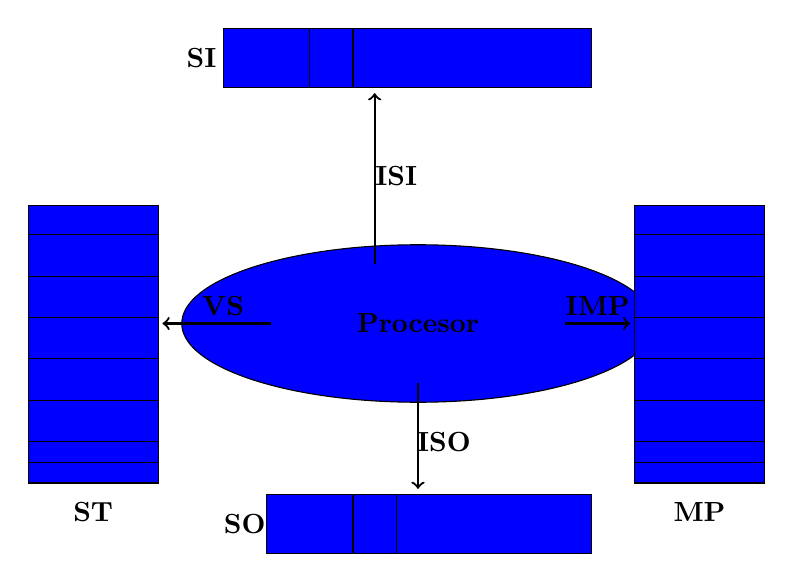
\begin{tikzpicture}[x=0.55cm, y=0.75cm]
\node at (-5,4.5) {\textbf{SI}};
\draw[black,fill=blue] (0,0) ellipse (3 cm and 1cm);
\draw[black,fill=blue] (-4.5,5) rectangle (-2.5,4);
\draw[black,fill=blue] (-2.5,5) rectangle (-1.5,4);
\draw[black,fill=blue] (-1.5,5) rectangle (4,4);
\node at (0,0) {\textbf{Procesor}};
\draw [thick, ->] (-1,1) -- (-1,3.9) node[anchor=south east] {};
\node at (-0.5,2.5) {\textbf{ISI}};
\draw[black,fill=blue] (-9,2) rectangle (-6,1.5);
\draw[black,fill=blue] (-9,1.5) rectangle (-6,0.8);
\draw[black,fill=blue] (-9,0.8) rectangle (-6,0.1);
\draw[black,fill=blue] (-9,0.1) rectangle (-6,-0.6);
\draw[black,fill=blue] (-9,-0.6) rectangle (-6,-1.3);
\draw[black,fill=blue] (-9,-1.3) rectangle (-6,-2);
\draw[black,fill=blue] (-9,-2) rectangle (-6,-2.35);
\draw[black,fill=blue] (-9,-2.35) rectangle (-6,-2.7);
\node at (-7.5,-3.2) {\textbf{ST}};
\draw[thick, ->] (-3.4,0) -- (-5.9,0) node[anchor=north west] {};
\node at (-4.5,0.3) {\textbf{VS}};
\draw[black,fill=blue] (-3.5,-2.9) rectangle (-1.5,-3.9);
\draw[black,fill=blue] (-1.5,-2.9) rectangle (-0.5,-3.9);
\draw[black,fill=blue] (-0.5,-2.9) rectangle (4,-3.9);
\node at (-4,-3.4) {\textbf{SO}};
\draw [thick, ->] (0,-1) -- (0,-2.8) {};
\node at (0.6,-2) {\textbf{ISO}};
\draw[black,fill=blue] (5,2) rectangle (8,1.5);
\draw[black,fill=blue] (5,1.5) rectangle (8,0.8);
\draw[black,fill=blue] (5,0.8) rectangle (8,0.1);
\draw[black,fill=blue] (5,0.1) rectangle (8,-0.6);
\draw[black,fill=blue] (5,-0.6) rectangle (8,-1.3);
\draw[black,fill=blue] (5,-1.3) rectangle (8,-2);
\draw[black,fill=blue] (5,-2) rectangle (8,-2.35);
\draw[black,fill=blue] (5,-2.35) rectangle (8,-2.7);
\node at (6.5,-3.2) {\textbf{MP}};
\draw [thick, ->] (3.4,0) -- (4.9,0) {};
\node at (4.15,0.3) {\textbf{IMP}};
\end{tikzpicture}
\end{center}
\end{frame}



\begin{frame}{Maşina de analiză predictivă}
\begin{itemize}

\item \textbf{Procesorul} este unitatea centrală virtuală care interpretează programele şi le execută.

\item \textbf{SI} este şirul de intrare cu indicele  \underline{ISI} care marchează poziţia atomului lexical curent de analizat

\item \textbf{SO} este şirul de ieşire cu indicele  \underline{ISO} care marchează ultimul element introdus în șir

\item \textbf{ST} este o memorie de tip stivă, cu  \underline{VS} vârful stivei

\item \textbf{MP} este memoria program, accesibilă doar la citire, cu \underline{IMP} indicele instrucţiunii curente

\end{itemize}
\end{frame}



\begin{frame}{Maşina de analiză predictivă}
\begin{itemize}
\item Procesorul citește programele din MP şi le executa la fel ca şi procesorul oricărui calculator real
\item
El poate citi un atom din SI, poate scrie un atom lexical în SO şi poate scrie sau citi din vârful stivei ST

\end{itemize}
\end{frame}



\begin{frame}{Maşina de analiză predictivă}
MAP recunoaşte şi execută \textbf{patru instrucţiuni}:      

\begin{enumerate}

\item \textcolor{red}{Instructiunea de \textbf{test (V)}}

\item \textcolor{red}{Instructiunea de \textbf{apel cu revenire (A)}}

\item \textcolor{red}{Instrucţiunea \textbf{adevărat (T)}}

\item \textcolor{red}{Instrucţiunea \textbf{fals (F)}}

\end{enumerate}
\end{frame}



\begin{frame}{Instrucțiunea de test}

\begin{center}
$V(a), E_{1}, E_{2}$
\end{center}

\begin{itemize}
\item 
Instrucţiunea de test face \textbf{verificarea identității dintre atomul lexical curent din SI şi atomul lexical indicat între paranteze}, adică a. 

\item 
În caz de identitate:

\begin{itemize}
\item
a este scris în  şirul SO
\item
se avansează în SI 
\item
şi se continuă execuţia cu instrucţiunea $E_{1}$
\end{itemize}

\item 
În caz contrar:
\begin{itemize}
\item
se continuă execuţia cu instrucţiunea $E_{2}$
\end{itemize}
\end{itemize}
\end{frame}



\begin{frame}{Instrucțiunea de test}

\begin{center}
$V(a), E_{1}, E_{2}$
\end{center}

\begin{itemize}
\item 
Dacă câmpurile $E_{1}$ si $E_{2}$ sunt vide, atunci execuţia se continuă cu următoarea instrucţiune din MP

\item 
$E_{1}$ şi $E_{2}$ pot fi etichete ale unor instrucţiuni din MP, sau pot fi una dintre instrucţiunile T şi F
\end{itemize}
\end{frame}



\begin{frame}{Instrucțiunea de apel cu revenire}

\begin{center}
$A(E), E_{1}, E_{2}$
\end{center}

\begin{itemize}
\item 
Permite execuția secvenţei de program de la eticheta E

\item 
Înainte de execuţia primei instrucţiuni de la eticheta E, se salvează starea maşinii de analiză, adică tripletul (ISI, ISO, IMP), în ST

\item 
Dacă returul din secvenţă se face cu instrucţiunea adevarat (T), atunci se va executa în continuare instructiunea $E_{1}$

\item 
Dacă returul din secvenţă se face cu instrucţiunea fals (F), atunci se va executa în continuare instrucţiunea $E_{2}$

\end{itemize}
\end{frame}



\begin{frame}{Instrucțiunea de apel cu revenire}

\begin{center}
$A(E), E_{1}, E_{2}$
\end{center}

\begin{itemize}
\item 
Dacă câmpurile $E_{1}$ și $E_{2}$ sunt vide, atunci execuţia se continuă cu următoarea instrucţiune din MP

\item 
$E_{1}$ şi $E_{2}$ pot fi etichete ale unor instrucţiuni din MP, sau pot fi una dintre instrucţiunile T şi F
\end{itemize}
\end{frame}



\begin{frame}{Algoritmul mașinii de analiză predictivă}
\begin{tabbing}
	ISI,ISO,VS,IMP$\leftarrow$0\\
	repeta \=\\
            \> daca \= MP(IMP)=A \+ \\
                 \> atunci *A \\
            altfel *V
\end{tabbing}
\end{frame}



\begin{frame}{Instrucţiunea V}
\begin{tabbing}
		k=1\\
        daca \= MP(IMP+1)=SI(ISI)\\
                 \> atunci \= \+ \\
                      \> ISI$\leftarrow$ ISI+1 \+ \\
                         SO(ISO)$\leftarrow$MP(IMP+1)\\
                    	 ISO$\leftarrow$ISO+1\\
                    	 K1$\leftarrow$IMP+2\\ \- \\
                         altfel \+ \\
                                K1$\leftarrow$IMP+3 \-\- \\
                
\end{tabbing}
\end{frame}



\begin{frame}{Intrucțiunea V}
\begin{tabbing}
repeta \= pana cand k=0\\
	   \> daca \= MP(K1)=blank \+ \\
		       \> atunci IMP = IMP + 4; K=0\\
		  altfel\\
			\> daca \= MP(K1)=T \+ \\
				\> atunci *T\\
				altfel \+ \\
					daca \= MP(K1)=F \+ \\
						atunci *F \-\\
				 altfel IMP = MP(K1); K=0\\
\end{tabbing}
\end{frame}



\begin{frame}{Instrucțiunea A}

ST(VS)=ISI,ISO,IMP

VS=VS+3

IMP $\leftarrow$ MP(IMP+1)\\
\end{frame}



\begin{frame}{Intrucțiunea F}
\begin{tabbing}

daca \= VS=0  \\
     \> atunci *esec \\
altfel \+ \\
       IMP=ST(VS)\\
          ISO=ST(VS)\\
          ISI=ST(VS)\\
          K1=IMP+3\\
          VS=VS-3

\end{tabbing}
\end{frame}



\begin{frame}{Intrucțiunea T}
\begin{tabbing}
daca VS != 0 atunci \\
\hspace*{1cm} IMP = ST(VS) \\
\hspace*{1cm} VS = VS-3 \\
\hspace*{1cm} SO(ISO) = MP(IMP+1) \\
\hspace*{1cm} ISO = ISO + 1 \\
\hspace*{1cm} K1 = IMP + 2 \\
altfel daca VS=0 atunci \\
\hspace*{1cm} daca \ SI(ISI-1) = $\epsilon $ \\
\hspace*{2cm} atunci \ *succes \\
\hspace*{1cm} altfel \ *esec \\
\end{tabbing}
\end{frame}



\begin{frame}{Algoritmul mașinii de analiză predictivă}

Pentru a putea utiliza mașina de analiză predictivă:

\begin{itemize}
\item
gramatica generatoare a limbajului ţintă \textbf{trebuie să îndeplinească numai prima condiţie} dintre cele cerute pentru analiza sintactică predictivă
\end{itemize}

\end{frame}



\begin{frame}{Exemplu}
Fie gramatica G=$\langle \Sigma, V_N, X, P \rangle$, unde:

\begin{itemize}
\item
$\sum$=\{+,*,-,a,(,)\}
\item
$V_N$=\{X,Y,Z,W\}
\item
X
\item
$P$=\{

\hspace{1cm} $X \rightarrow Y$ \\
\hspace{1cm} $Y \rightarrow Z+W $ \\
\hspace{1cm} $Y \rightarrow Z*W $ \\
\hspace{1cm} $Y \rightarrow Z$ \\
\hspace{1cm} $Z \rightarrow -W$ \\
\hspace{1cm} $Z \rightarrow W$ \\
\hspace{1cm} $W \rightarrow a$ \\
\hspace{1cm} $W \rightarrow (Y)$
\}
\end{itemize}

\begin{itemize}
\item
Scrieti programul mașinii de analiză predictivă pentru limbajul definit de gramatica G.

\item
Analizați propoziția \textcolor{red}{a+(-a)}.
\end{itemize}
\end{frame}



\begin{frame}{Exemplu}
\begin{center}
\begin{tabular*}{\textwidth}{@{\extracolsep{\fill} } | c | c | c | c | c | c | c | }
\hline
	              & + & * & - & a & (  & )   \\ \hline
X				  &   &   & Y & Y &  Y &     \\ \hline
Y	              &   &   & Z+W & Z+W & Z+W &   \\
				  &   &   & Z*W & Z*W & Z*W &	 \\
				  &   &   & Z & Z & Z & \\ \hline
Z	              &   &   & -W & W & W &      \\ \hline
W			      &   &   &   & a &(Y)  &   \\ \hline 
\end{tabular*}
\end{center}
\end{frame}



\begin{frame}{Exemplu}

%%%%%%%%%%%slide-urile 32%%%%%%%%%%%%%%%%

00$\ $     X:  \textbf{A}(Y),  $\ $,F

04$\ \ \ $  :  \textbf{V}($\epsilon$),T,F

08$\ $     Y:  \textbf{A}(Z),$\ $,F

12$\ \ \ $  :  \textbf{V}(+),Y1,$\ $

16$\ \ \ $  :  \textbf{V}(*),Y1,T

20   Y1:  \textbf{A}(W),T,F 

24$\ $     Z:  \textbf{V}(-),$\ $,$\ $

28$\ \ \ $  :  \textbf{A}(W),T,F

32$\ $    W:  \textbf{V}(a),T,$\ $

36$\ \ \ $  :  \textbf{V}((),$\ $,F

40$\ \ \ $  :  \textbf{A}(Y),$\ $,F

44$\ \ \ $  :  \textbf{V}()),T,F

\end{frame}



\begin{frame}{Exemplu}
\begin{table}[H]
	\centering
	\begin{tabular}{|l c c c c r|}
		\hline
			\textbf{SI} & \textbf{ISI} & \textbf{ISO} & \textbf{IMP} & \textbf{SO} & \textbf{ST} \\
		\hline
			$\underline{a}+(-a)\$$ & 0 & 0 & 0 & - & \\
		\hline
			$\underline{a}+(-a)\$$ & 0 & 0 & 0 & - & (0,0,0) \\
		\hline
			$\underline{a}+(-a)\$$ & 0 & 0 & 8 & - & (0,0,0)(0,0,8) \\
		\hline
			$\underline{a}+(-a)\$$ & 0 & 0 & 24 & - & (0,0,0)(0,0,8) \\
		\hline
			$\underline{a}+(-a)\$$ & 0 & 0 & 28 & - & (0,0,0)(0,0,8)(0,0,28) \\
		\hline
			$\underline{a}+(-a)\$$ & 0 & 0 & 32 & - & (0,0,0)(0,0,8)(0,0,28) \\
		\hline
			$a\underline{+}(-a)\$$ & 1 & 2 & 28 & aw & (0,0,0)(0,0,8) \\
		\hline
			$a\underline{+}(-a)\$$ & 1 & 3 & 8 & awz & (0,0,0) \\
		\hline
			$a\underline{+}(-a)\$$ & 1 & 3 & 12 & awz & (0,0,0) \\
		\hline 
			
		\end{tabular}
	\end{table}
\end{frame}



\begin{frame}{Exemplu}

\begin{table}[H]
	\centering
    \scalebox{0.8}{
	\begin{tabular}{|l c c c c r|}
		\hline
			\textbf{SI} & \textbf{ISI} & \textbf{ISO} & \textbf{IMP} & \textbf{SO} & \textbf{ST} \\
		\hline
			$a+\underline{\textbf{(}}-a)\$$ & 2 & 4 & 20 & awz+ & (0,0,0)\\
		\hline
			$a+\underline{\textbf{(}}-a)\$$ & 2 & 4 & 32 & awz+ & (0,0,0)(2,2,20) \\
		\hline
			$a+\underline{\textbf{(}}-a)\$$ & 2 & 4 & 36 & awz+ & (0,0,0)(2,2,20) \\
		\hline
			$a+(\underline{\textbf{-}}a)\$$ & 3 & 5 & 40 & awz+( & (0,0,0)(2,2,20) \\
		\hline
			$a+(\underline{\textbf{-}}a)\$$ & 3 & 5 & 8 & awz+( & (0,0,0)(2,2,20)(3,3,40) \\
		\hline
			$a+(\underline{\textbf{-}}a)\$$ & 3 & 5 & 24 & awz+( & (0,0,0)(2,2,20)(3,3,40)(3,3,8) \\
		\hline
			$a+(\textbf{-} \underline{a})\$$ & 4 & 6 & 28 & awz+(- & (0,0,0)(2,2,20)(3,3,40)(3,3,8) \\
		\hline
			$a+(\textbf{-}\underline{a})\$$ & 4 & 6 & 32 & awz+(- & (0,0,0)(2,2,20)(3,3,40)(3,3,8)(4,4,28) \\
		\hline
			$a+(-a\underline{\textbf{)}}\$$ & 5 & 8 & 28 & awz+(-aw & (0,0,0)(2,2,20)(3,3,40)(3,3,8) \\
		\hline 			
		\end{tabular}
		}
	\end{table}
\end{frame}



\begin{frame}{Exemplu}
\begin{table}[H]
\centering
\scalebox{0.8}{
\begin{tabular}{|l c c c c r|}
\hline
\textbf{SI} & \textbf{ISI} & \textbf{ISO} & \textbf{IMP} & \textbf{SO} & \textbf{ST} \\
\hline
$a+(-a\underline{)}\$$ & $5$&$9$ & $8$ & $awz+(-awz$ & $(0,0,0)(2,2,20)(3,3,40)$ \\
\hline
$a+(-a\underline{)}\$$ & $5$ & $9$ & $12$&$awz+(-awz$ & $(0,0,0)(2,2,20)(3,3,40)$\\
\hline
$a+(-a\underline{)}\$$ & $5$ & $9$ & $16$&$awz+(-awz$ & $(0,0,0)(2,2,20)(3,3,40)$\\
\hline
$a+(-a\underline{)}\$$ & $5$ & $10$ & $40$&$awz+(-awzy$ & $(0,0,0)(2,2,20)$ \\
\hline
$a+(-a)\underline{\$}$ & $6$ & $11$ & $20$&$awz+(-awzy)$ & $(0,0,0)$ \\
\hline
$a+(-a)\underline{\$}$ & $6$ & $12$ & $0$&$awz+(-awzy)w$ & $-$ \\
\hline
$a+(-a)\underline{\$}$ & $6$ & $13$ & $4$&$awz+(-awzy)wv$ & $-$ \\
\hline
\end{tabular}
}
\end{table}
\end{frame}



\begin{frame}{Analiza sintactica descendentă cu reveniri}
\begin{itemize}
\item 
Analiza sintactică descendetă cu reveniri este o implementare deterministă a analizei sintactice predictive

\begin{figure}
\centering
\includegraphics[scale=0.8]{img/asdr}
\end{figure}
\end{itemize}
\end{frame}



\begin{frame}{Analiza sintactica descendentă cu reveniri}
\begin{itemize}
\item 
Si - șirul de intrare (conține atomii lexicali obtinuți în urma etapei de analiză lexicală)

\item 
isi - indice pentru Si

\item 
St1 - stiva (acces LIFO) pentru construirea arborelui sintactic

\item 
ist1 - vârful stivei St1

\item 
St2 - stiva de retur

\item 
Ist2 - vârful stivei St2
\end{itemize}
\end{frame}



\begin{frame}{Analiza sintactica descendentă cu reveniri}
Configurația automatului finit cu memorie:

(s, i, $\alpha$, $\beta$ )

\begin{itemize}
\item
\textbf{s} - starea automatului finit, care poate fi:

\begin{itemize}
\item
q (stare normală)
\item
b (stare de revenire)

\item
e (stare de eroare)

\item
a (stare de acceptare) 
\end{itemize}

\item
\textbf{j} - indicele șirurului de intrare

\item
\textbf{$\alpha$} - șirul din  stiva St2, formată din atomi lexicali deja recunoscuți în șirul de intrare și din indicii regulilor de producție utilizate în relațiile de derivare

\item
\textbf{$\beta$} - șirul din stiva St1
\end{itemize}
\end{frame}



\begin{frame}{Analiza sintactica descendentă cu reveniri}
\begin{enumerate}
\item 
\textbf{configurația inițială}

(q, 0, $\epsilon$, S)

\item 
\textbf{expandarea}

(q, j, $\alpha$, A$\beta$) $\rightarrow$ (q, j, $\alpha$A1, $\alpha_1\beta$)

unde A1: A $\rightarrow$ $\alpha_1$ este prima regulă de producție pentru neterminalul A din vârful stivei St1 (A va fi expandat conform primei alternative)

\item 
\textbf{avans}

(q, j, $\alpha$, a$\beta$) $\rightarrow$ (q, j+1, $\alpha$a, $\beta$), 

cand în vârful stivei St1 se află un terminal identic cu cel din poziția curentă (j) a șirului de intrare

\end{enumerate}
\end{frame}



\begin{frame}{Analiza sintactica descendentă cu reveniri}
\begin{enumerate}
\item[4.]
\textbf{necoincidența}

(q, j, $\alpha$, i$\beta$) $\rightarrow$ (b, j, $\alpha$, i$\beta$)

\begin{itemize}
\item
când în vârful stivei St1 se află un terminal care nu este identic cu cel din poziția curentă (j) a șirului de intrare
\end{itemize}

\item[5.]
\textbf{revenire}

\begin{enumerate}
\item[5.1]
(b, j, $\alpha$i, $\beta$) $\rightarrow$ (b, j-1, $\alpha$, i$\beta$)

\begin{itemize}
\item
când în vârful stivei St2 se află un terminal
\item
pasul 5.1 se repetă atâta timp cât se află un terminal în vârful stivei St2
\end{itemize}

\item[5.2]
(b, j, $\alpha A_i$, $\alpha_i\beta$) $\rightarrow$ (q, j, $\alpha A_{i+1}$, $\alpha_{i+1}\beta$)

\begin{itemize}
\item
se sare la pasul 3
\end{itemize}

\item[5.3]
(b, j, $\alpha A_n$, $\alpha_n\beta$) $\rightarrow$ (b, j, $\alpha$, A$\beta$)

\begin{itemize}
\item
se sare la pasul 5.1
\end{itemize}


\end{enumerate}
\end{enumerate}
\end{frame}



\begin{frame}{Analiza sintactica descendentă cu reveniri}
\begin{enumerate}
\item[6]
\textbf{eșec}

(b, j, $\alpha$, S$\beta$) $\rightarrow$ (e, j, $\alpha$, S$\beta$)

\item[7]
\textbf{succes}

(q, n+1, $\alpha$, $\epsilon$) $\rightarrow$ (a, n+1, $\alpha$, $\epsilon$)
\end{enumerate}
\end{frame}



\begin{frame}{Analiza sintactica descendentă cu reveniri}

Pentru a putea utiliza analiza sintactică cu reveniri:

\begin{itemize}
\item
gramatica generatoare a limbajului ţintă \textbf{trebuie să îndeplinească numai prima condiţie} dintre cele cerute pentru analiza sintactică predictivă
\end{itemize}

\end{frame}



\begin{frame}{Exemplu}
Fie gramatica G=$\langle \Sigma, V_N, S, P \rangle$, unde:

\begin{itemize}
\item
$\sum$=\{a,b,c\}
\item
$V_N$=\{S,A,B\}
\item
S
\item
$P$=\{

\hspace{1cm} $(S1)	S \rightarrow Ab$

\hspace{1cm} $(S2)	S \rightarrow Ac$

\hspace{1cm} $(A1)	A \rightarrow a$

\hspace{1cm} $(A2)	A \rightarrow bAB$

\hspace{1cm} $(B1)	B \rightarrow a$

\}
\end{itemize}

Folosind automatul finit cu memorie cu reveniri, analizaţi propoziţiile:

\begin{itemize}
\item
bbaaab

\item
bbaabab

\end{itemize}
\end{frame}



\begin{frame}{Exemplu}

$( q, 1, \epsilon ,S )$

$\vdash (2) \hspace{1cm} (q, 1, S1, Ab) \hspace{2cm} //expandare$

$\vdash (2) \hspace{1cm} (q, 1, S1A1, ab) \hspace{1.65cm} //st2(ist2)\neq si(isi)
) $ 

$\vdash (4) \hspace{1cm}(b,1,S1A1, ab) \hspace{1.65cm} //necoincidenta$ 

$\vdash (5.2)\hspace{0.7cm}(q, 1, S1A2, bABb) \hspace{1.1cm} //revernire$ 

$\vdash (3) \hspace{1cm}(q, 2, S1A2b, ABb) \hspace{1.1cm} //avans)$ 

$\vdash (2) \hspace{1cm}(q, 2, S1A2bA1, aBb) \hspace{0.75cm} //expandare \ A1 \to a)$ 

$\vdash (4) \hspace{1cm}(b, 2, S1A2bA1, aBb) \hspace{0.75cm} {//necoincidenta})$ 

$\vdash (5.2) \hspace{0.7cm}(q, 2, S1A2bA2, bABBb) \hspace{0.25cm} {//revenire})$ 

\end{frame}



\begin{frame}{Exemplu}

$\vdash  (3)\hspace{1cm}	(q, 3, S1A2bA2b, ABBb)	      \hspace{2cm}    //avans	$
$\vdash  (2)\hspace{1cm}	(q, 3, S1A2bA2bA1, aBBb)      \hspace{1.6cm}  //expandare$
$\vdash  (3)\hspace{1cm}	(q, 4, S1A2bA2bA1a, BBb)      \hspace{1.6cm}  //avans$
$\vdash  (2)\hspace{1cm}	(q, 4, S1A2bA2bA1aB1, aBb)    \hspace{1.2cm}  //expandare$
$\vdash  (3)\hspace{1cm}	(q, 5, S1A2bA2bA1aB1a, Bb)    \hspace{1.2cm}  //avans$
$\vdash  (2)\hspace{1cm}	(q, 5, S1A2bA2bA1aB1aB1, ab)  \hspace{0.8cm}  //expandare$
$\vdash  (3)\hspace{1cm}	(q, 6, S1A2bA2bA1aB1aB1a, b)  \hspace{0.75cm}  //avans$
$\vdash  (3)\hspace{1cm}	(q, 7, S1A2bA2bA1aB1aB1ab, \$)\hspace{0.7cm}  //avans$
$\vdash  (7)\hspace{1cm}	(q, 7, S1A2bA2bA1aB1aB1ab, \epsilon) \hspace{0.7cm} //succes$
$\vdash  (7)\hspace{1cm}	(a, 7, S1A2bA2bA1aB1aB1ab, \epsilon)$

\end{frame}



\begin{frame}{Analiza sintactică LL(1)}
\begin{itemize}
\item
Analiza LL(k) 
\begin{itemize}
\item
tip de analiză sintactică descendentă
\item
analizează intrarea de la stânga la dreapta (\color{red}L\color{black}eft to right)
\item
construieşte o derivare stânga pentru aceasta (\color{red}{L}\color{black}eftmost derivation)
\item
de aici denumirea de \color{red}{LL}\color{black}
\item
decizia de a folosi a anumită regulă de producţie pentru a expanda vâtful stivei se ia \color{red}{după inspectarea în avans a unui număr de k atomi lexicali} \color{black} din şirul de intrare
\item
de aici denumirea de \color{red}{LL(k)}\color{black}
\item
în consencinţă, analiza nu foloseşte reveniri
\end{itemize}
\end{itemize}
\end{frame}



\begin{frame}{Analiza sintactică LL(1)}
\begin{itemize}
\item
Dacă pentru a anumită gramatică generatoare G se poate defini un analizor LL(k), atunci gramatica se numeşte \textbf{gramtică LL(k)}

\item 
Limbajul definit printr-o astfel de gramatică se numeşte limbaj LL(k)

\item
Cele mai răspândite sunt \textbf{gramaticile LL(1)}
\begin{itemize}
\item
analizorul trebuie să inspecteze doar următorul atom lexical din şirul de intrare pentru a putea lua deciziile de analiză
\end{itemize}
\end{itemize}
\end{frame}



\begin{frame}{Analiza sintactică LL(1)}
Fie gramatica G=$\langle \Sigma, V_N, S, P \rangle$, unde:

\begin{itemize}
\item
$\sum$=\{a,b,c\}
\item
$V_N$=\{S,A\}
\item
S
\item
$P$=\{

\hspace{1cm} (1.1) S $\rightarrow$ \underline{a}SAc

\hspace{1cm} (1.2) S $\rightarrow$ \underline{$\epsilon$}

\hspace{1cm} (2.1) A $\rightarrow$ \underline{b}A

\hspace{1cm} (2.2) A $\rightarrow$ \underline{$\epsilon$}

\}
\end{itemize}

\begin{figure}[H]
\centering
\begin{tabular}{ | c | c |  c |  c |}
\hline
& a & b & c \\ [0.5ex] 
 \hline
 S & 1.1 & 1.2 & 1.2\\
 A & & 2.1 & 2.2\\
 \hline
 \end{tabular}
\end{figure}
\end{frame}



\begin{frame}{Analiza sintactică LL(1)}

\begin{itemize}
\item
Succesiunea de relații de mișcare ale automatului finit cu memorie, conform algoritmului de analiză LL(1) pentru propoziția: \textbf{aabcc}
\end{itemize}

$(q, 0, S) $ \hspace{2cm} - a următorul atom, deci alegem 1.1

$\vdash (q, 0, aSAc)$

$\vdash (q, 1, SAc)$ \hspace{1.2cm} - a următorul atom, deci alegem 1.1

$\vdash (q, 1, aSAcAc) $

$\vdash (q, 2, SAcAc)$ \hspace{0.8cm} - b următorul atom, deci alegem 1.2

$\vdash (q, 2, AcAc)$ \hspace{1cm} - b următorul atom, deci alegem 2.1

\end{frame}



\begin{frame}{Analiza sintactică LL(1)}

$\vdash (q, 2, bAcAc)$

$\vdash (q, 3, AcAc)$ \hspace{1.2cm} - c următorul atom, deci alegem 2.2

$\vdash (q, 3, cAc)$

$\vdash (q, 4, Ac)$ \hspace{1.6cm} - c următorul atom, deci alegem 2.2

$\vdash (q, 4, c)$ 

$\vdash (q, 5, \epsilon)$

\end{frame}



\begin{frame}{Gramatici LL(1)}

\begin{itemize}
\item
Pentru a putea construi un analizor LL(1) pentru o gramatică $G=\langle \Sigma, V_N, S, P \rangle$, aceasta trebuie să fie o \textbf{gramatică LL(1)}

\item
Condiţii necesare şi suficiente pentru ca o gramatică independentă de context să fie o gramatică LL(1):

$\forall A \in V_N, A \to \alpha{_1} | \alpha{_2} | \dots | \alpha{_n} \in P$

\begin{itemize}
\item
1. $FIRST^+(\alpha{_i}) \cap FIRST^+ (\alpha{_j}) =\emptyset, \forall i \neq j$

\item
2. $FOLLOW^+(A) \cap FIRST^+ (\alpha{_j}) = \emptyset, \forall i, \alpha{_i} \Rightarrow^{*} \epsilon \wedge \forall j$
\end{itemize}
\end{itemize}
\end{frame}



\begin{frame}{$FIRST^+$}

Pentru fiecare $A \to \alpha{_1} | \alpha{_2} | \dots | \alpha{_n} \in P, A \in V_N, \forall i \  \alpha_i \neq \epsilon$

\begin{itemize}
\item
$FIRST^+(\alpha_i) = \{ a \in \Sigma | \alpha_i \Rightarrow^* a \gamma, \gamma \in V^{*} \}$

\item
Dacă $\alpha_i \Rightarrow^* \epsilon$, atunci trebuie să se ţină cont de ceea ce urmează după A

\item
(În cazul metodei LL1 se analizează în avans \textbf{un singur }atom lexical.)
\end{itemize}
\end{frame}



\begin{frame}{$FOLLOW^+$}

Pentru $A \to \epsilon \in P, A \in V_N$

\begin{itemize}
\item
$FOLLOW^+(A) = \{ a  \in \Sigma | (S \Rightarrow^* \alpha A a \beta, \alpha,\beta \in V^{*}) \vee ( S \Rightarrow^* xAY, a \in FIRST^+(Y), x \in \Sigma^*) \vee (S \Rightarrow^* \alpha A, a \in FOLLOW^+(S)) \}$

\item
(În cazul metodei LL1 se analizează în avans \textbf{un singur }atom lexical.)
\end{itemize}
\end{frame}



\begin{frame}{Analiza sintactică LL(1)}

Pentru a putea construi un analizor sintactic LL(1):

\begin{itemize}
\item
gramatica generatoare a limbajului ţintă \textbf{trebuie să îndeplinească ambele condiţii} cerute pentru analiza sintactică predictivă
\end{itemize}

\end{frame}



\begin{frame}{Analiza sintactică LL(1)}

Etapele analizei sintactice LL(1):

\begin{itemize}
\item
Construirea analizorului sintactic LL(1):

\begin{itemize}
\item
Modificarea gramaticii astfel încât să respecte cele două condiții cerute pentru analiza sintactică predictivă
\item
Calcularea mulțimilor de simboli directori (mulțimile $FIRST^+$ sau $FOLLOW^+$) 
\item
Verificarea îndeplinirii condițiilor pentru ca G să fie o gramatică LL(1)
\item
Construirea tabelei de analiză sintactică
\item
Implementarea analizorului sintactic LL(1)
\end{itemize}

\item
Analiza propriu-zisă a unei propoziții
\end{itemize}

\end{frame}



\begin{frame}{Exemplu}
Fie gramatica G=$\langle \Sigma, V_N, E, P \rangle$, unde:

\begin{itemize}
\item
$\sum$=\{+,*,(,),a\}
\item
$V_N$=\{E,T,F\}
\item
E
\item
$P$=\{

\hspace{1cm} E$\to$E+T$\mid$T\\
\hspace{1cm} T$\to$T*F$\mid$F\\
\hspace{1cm} F$\to$a$\mid$(E)\\
\}
\end{itemize}

\begin{itemize}
\item
Gramatica folosește \textbf{recursivitatea stânga}
\begin{itemize}
\item
pentru a se putea construi un analizor sintactic LL(1) (descendent), ea trebuie să fie modificată
\end{itemize}
\end{itemize}
\end{frame}



\begin{frame}{Exemplu}
Gramatica modificată este G=$\langle \Sigma, V_N, E, P \rangle$, unde:

\begin{itemize}
\item
$\sum$=\{+,*,(,),a\}
\item
$V_N$=\{E,E1,T,T1,F\}
\item
E
\item
$P$=\{

\hspace{1cm} 1. E$\rightarrow$TE$_1$

\hspace{1cm} 2. E$_1\rightarrow+$TE$_1$

\hspace{1cm} 3. E$_1\rightarrow \varepsilon$

\hspace{1cm} 4. T$\rightarrow$FT$_1$

\hspace{1cm} 5. T$_1\rightarrow *$FT$_1$

\hspace{1cm} 6. T$_1 \rightarrow \varepsilon$

\hspace{1cm} 7. F$ \rightarrow$(E)

\hspace{1cm} 8. F$ \rightarrow$a

\}
\end{itemize}

\end{frame}



\begin{frame}{Exemplu}
\begin{itemize}
\item[$\blacktriangleright$]
\textcolor{blue}{Se calculează mulțimile de simboli directori:}
\item[$\blacktriangleright$]
\textbf{\textcolor{red}{D$_1$}=FIRST$^+$(TE$_1$)=FIRST$^+$(F)=\textcolor{red}{$\lbrace$(,a$\rbrace$}}
\item[$\blacktriangleright$]
\textbf{\textcolor{red}{D$_2$}=FIRST$^+$($+$TE$_1$)=\textcolor{red}{$\lbrace+\rbrace$}}
\item[$\blacktriangleright$]
\textbf{\textcolor{red}{D$_3$}=FOLLOW$^+$(E$_1$)=FOLLOW$^+$(E)=\textcolor{red}{$\lbrace$)$\rbrace$}}
\item[$\blacktriangleright$]
\textbf{\textcolor{red}{D$_4$}=FIRST$^+$(FT$_1$)=FIRST$^+$(F)=\textcolor{red}{$\lbrace$(,a$\rbrace$}}
\item[$\blacktriangleright$]
\textbf{\textcolor{red}{D$_5$}=FIRST$^+$($*$FT$_1$)=\textcolor{red}{$\lbrace*\rbrace$}}
\item[$\blacktriangleright$]
\textbf{\textcolor{red}{D$_6$}=FOLLOW$^+$(T$_1$)=FOLLOW$^+$(T)=}

\textbf{FIRST$^+$(E$_1) \cup$FOLLOW$^+$(E)=$\lbrace+\rbrace \cup \lbrace)\rbrace$=\textcolor{red}{$\lbrace+$,)$\rbrace$}}
\item[$\blacktriangleright$]
\textbf{\textcolor{red}{D$_7$}=FIRST$^+$((E))=\textcolor{red}{$\lbrace(\rbrace$}}
\item[$\blacktriangleright$]
\textbf{\textcolor{red}{D$_8$}=FIRST$^+$(a)=\textcolor{red}{$\lbrace a\rbrace$}}
\end{itemize}
\end{frame}



\begin{frame}{Exemplu}
\begin{itemize}
\item[$\blacktriangleright$]
\textcolor{blue}{Se verifică îndeplinirea condițiile pentru ca G să fie o gramatică LL(1): }
\item[$\blacktriangleright$]
\tab \textbf{D$_2 \cap$D$_3$ = $\emptyset$}
\item[$\blacktriangleright$]
\tab \textbf{D$_5 \cap$D$_6$ = $\emptyset$}
\item[$\blacktriangleright$]
\tab \textbf{D$_7 \cap$D$_8$ = $\emptyset$}
\item[$\blacktriangleright$]
\textbf{Rezultă faptul că gramatica este o gramatica \textbf{LL(1)}}
\end{itemize}
\end{frame}



\begin{frame}{Tabela de analiză sintactică}
\begin{itemize}
\item
pe baza mulțimilor FIRST și FOLLOW calculate, se generează tabela de analiză sintactică
\end{itemize}

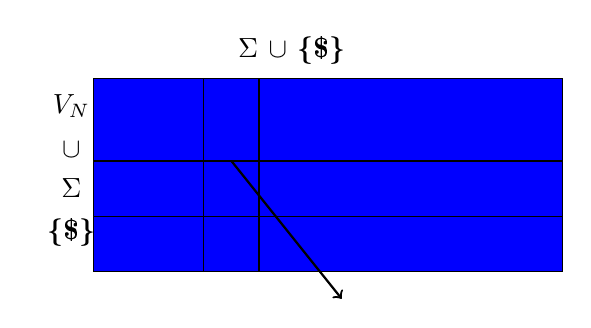
\begin{tikzpicture}[x=0.7cm, y=0.7cm]
\node at (-1,6) {\textbf{ $\Sigma$ $\cup$ \{\textdollar\}}};
\draw[black,fill=blue] (-4.5,5.5) rectangle (-2.5,4);
\draw[black,fill=blue] (-2.5,5.5) rectangle (-1.5,4);
\draw[black,fill=blue] (-1.5,5.5) rectangle (4,4);
\draw[black,fill=blue] (-4.5,3) rectangle (-2.5,4);
\draw[black,fill=blue] (-2.5,3) rectangle (-1.5,4);
\draw[black,fill=blue] (-1.5,3) rectangle (4,4);
\draw[black,fill=blue] (-4.5,2) rectangle (-2.5,4);
\draw[black,fill=blue] (-2.5,2) rectangle (-1.5,4);
\draw[black,fill=blue] (-1.5,2) rectangle (4,4);
\node at (-5,5) {\textbf{ $V_{N}$ }};
\node at (-5,4.2) {\textbf{ $\cup$ }};
\node at (-5,3.5) {\textbf{ $\Sigma$ }};
\node at (-5,2.7) {\textbf{ \{\textdollar\} }};
\draw[black,fill=blue] (-4.5,2) rectangle (-2.5,3);
\draw[black,fill=blue] (-2.5,2) rectangle (-1.5,3);
\draw[black,fill=blue] (-1.5,2) rectangle (4,3);
\draw [thick, ->] (-2,4) -- (0,1.5) {};
\end{tikzpicture}

\begin{itemize}
\item
P - pop - scoate un simbol din stivă și înaintează în SI

\item
A - accept - propoziția este corectă

\item
E - error - propoziția este incorectă

\item
R n - replace - se inlocuiește VS cu partea dreaptă a regulii de producție $n$, după care $n$ se scrie în SO

\item
simbolul \textdollar reprezintă terminatorul de șir pentru SI
\end{itemize}
\end{frame}



\begin{frame}{Tabela de analiză sintactică}

\textbf{Algoritmul de construcție a tabelei de analiză sintactică:}

\begin{itemize}
\item
Pentru fiecare regulă de producție $n: A \rightarrow \alpha \in P$

\begin{itemize}
\item
pentru fiecare terminal din $FIRST^+(\alpha)$, se completează cu R n celula din tabelă corespunzătoare coloanei terminalului respectiv și liniei neterminalului A

\item
\textbf{sau}

\item
pentru fiecare terminal din $FOLLOW^+(A)$, se completează cu R n celula din tabelă corespunzătoare terminalului respectiv și liniei neterminalului A
\end{itemize}
\end{itemize}
\end{frame}



\begin{frame}{Analiza sintactica LL(1)}
\begin{itemize}
\item
pe baza tabelei de analiză sintactică se poate implementa un analizor sintactic determinist cu structura

\begin{figure}
\centering
\includegraphics[scale=0.7]{img/afsll1}
\end{figure}

%\begin{tikzpicture}[x=0.3cm]
%\node at (-5,4.5) {\textbf{SI}};
%\draw[black,fill=blue] (0,0) ellipse (3 cm and 1cm);
%\draw[black,fill=blue] (-4.5,5) rectangle (-2.5,4);
%\draw[black,fill=blue] (-2.5,5) rectangle (-1.5,4);
%\draw[black,fill=blue] (-1.5,5) rectangle (4,4);
%\node at (0,0) {\textbf{Procesor}};
%\draw [thick, ->] (-1,1) -- (-1,3.9) node[anchor=south east] {};
%\node at (-0.5,2.5) {\textbf{ISI}};
%\draw[black,fill=blue] (-9,2) rectangle (-6,1.5);
%\draw[black,fill=blue] (-9,1.5) rectangle (-6,0.8);
%\draw[black,fill=blue] (-9,0.8) rectangle (-6,0.1);
%\draw[black,fill=blue] (-9,0.1) rectangle (-6,-0.6);
%\draw[black,fill=blue] (-9,-0.6) rectangle (-6,-1.3);
%\draw[black,fill=blue] (-9,-1.3) rectangle (-6,-2);
%\draw[black,fill=blue] (-9,-2) rectangle (-6,-2.35);
%\draw[black,fill=blue] (-9,-2.35) rectangle (-6,-2.7);
%\node at (-7.5,-3.2) {\textbf{ST}};
%\draw[thick, ->] (-3.4,0) -- (-5.9,0) node[anchor=north west] {};
%\node at (-4.5,0.3) {\textbf{VS}};
%\draw[black,fill=blue] (-3.5,-2.9) rectangle (-1.5,-3.9);
%\draw[black,fill=blue] (-1.5,-2.9) rectangle (-0.5,-3.9);
%\draw[black,fill=blue] (-0.5,-2.9) rectangle (4,-3.9);
%\node at (-4,-3.4) {\textbf{SO}};
%\draw [thick, ->] (0,-1) -- (0,-2.8) {};
%\node at (0.6,-2) {\textbf{ISO}};
%\end{tikzpicture}

\end{itemize}
\end{frame}



\begin{frame}{Exemplu}

\begin{itemize}
\item 
pentru exemplul anterior, tabela de analiză sintactică este (celulele goale reprezintă E):
\end{itemize} 

\begin{table}[htb]
\begin{tabular}{|l|l|l|l|l|l|l|}
\hline
 &$a$  &$($ &$)$  &$+$  &$*$  &$\$$  \\ \hline
 $E$     &   R 1   &   R 1    &       &       &       &  \\ \hline
 $E_1$   &  &    &   R 3  &   R 2  &    &    R 3 \\ \hline
 $T$     &   R 4   &  R 4    &  &  &  &  \\ \hline
 $T_1$&  &  &   R 6  &   R 6  &  R 5   &    R 6 \\ \hline
 $F$&  R 8   &  R 7  &  &  &  &  \\ \hline
 $a$&    P &  &  &  &  &  \\ \hline
 $($&  &    P  &  &  &  &  \\ \hline
 $)$&  &  &    P &  &  &  \\ \hline
 $+$&  &  &  &   P  &  &  \\ \hline
 $*$&  &  &  &  &    P  &  \\ \hline
 $\$$&  &  &  &  &  &    A \\ \hline
\end{tabular}
\end{table}
\end{frame}



\begin{frame}{Algoritmul de analiză sintactică LL(1)}
\begin{tabbing}
sf $\leftarrow$ false\\

repeta \= pana cand sf = true\\
       \> daca St(VS) $\in \Sigma \  \wedge$ St(VS) = SI(ISI)  \\
       \> atunci \= \+ \\
       			  \> pop \\
       			  \> ISI = ISI + 1 \\

sau St(VS) $\in$ $\Sigma$ si St(VS) != SI(ISI) \\

atunci \\
\> error\\
\end{tabbing}
\end{frame}



\begin{frame}{Algoritmul de analiză sintactică LL(1)}
\begin{tabbing}
sau St(VS) = A$\ \in V_N$  \\

atunci \= \\

\> replace n \\
\> SO(ISO) = n \\
\> ISO = ISO +1 \\

sau St(VS) = SI(ISI) = \$    \\

atunci \\
\> accept\\
\> sf $\leftarrow$ true\\

altfel \\
\> error\\
\> sf $\leftarrow$ true\\
\end{tabbing}
\end{frame}



\begin{frame}{Analiza sintactică LL(1)}
\begin{itemize}
\item 
Modelul matematic al acestui tip de analiză rămâne automatul finit cu stivă 
\begin{itemize}
\item
un element suplimentar: șirul de iesire
\end{itemize}

\item Functia de tranzitie ($a,b,i,x \in \Sigma$):

\begin{itemize}
\item $f(q, a, a) = \{(q, \epsilon)\}$	pop

\item $f(q, \$, \$) = \{(a, \epsilon)\}$	accept

\item $f(q, b, A) = \{(q, \alpha)\}$	replace A $\rightarrow b\alpha$ conform tabelei de analiză sintactică

\item $f(q, i, x) = \{(e, \epsilon)\}$	error
\end{itemize}
\end{itemize}
\end{frame}



\begin{frame}{Analiza sintactică LL(1)}
\begin{itemize}
\item
\textbf{Configurația automatului:}

\begin{itemize}
\item
\textbf{(q,x,$\gamma$,y)}
\item
\textbf{q} - starea automatului
\item
\textbf{x} - șirul de intrare rămas de analizat
\item
\textbf{$\gamma$} - stiva
\item
\textbf{y} - șirul de iesire, format din indicii regulilor de producție utilizate în derivări
\end{itemize}

\item
\textbf{Configurații posibile:} ($a,b,i \in \Sigma,x \in \Sigma^*$)
\begin{itemize}
\item
(q,ax,a$\gamma$,y) $\rightarrow$ (q,x,$\gamma$,y) pop
\item
(q,ax,A$\gamma$,y) $\rightarrow$ (q,x,$\alpha\gamma$,yi) replace i, conform tabelei de analiză
\item
(q,\textdollar,\textdollar,y) $\rightarrow$ (a,$\epsilon$,$\epsilon$,y) accept
\item
$(q,bx,i\gamma,y) \rightarrow$ (e,$\epsilon$,$\epsilon$,y) error
\end{itemize}
\end{itemize}
\end{frame}



\begin{frame}{Exemplu}
Succesiunea relațiilor de mișcare pentru analiza propoziției \textbf{a * a + a} de către automatul construit în cadrul exemplului:

$(q,a*a+a\textdollar,E\textdollar,\epsilon)$

$\vdash^{r} (q,a*a+a\textdollar,TE_{1}\textdollar,1)$ 

$\vdash^{r} (q,a*a+a\textdollar,FT_{1}E_{1}\textdollar,14)$

$\vdash^{r} (q,a*a+a\textdollar,aT_{1}E_{1}\textdollar,148)$

$\vdash^{p} (q,*a+a\textdollar,FT_{1}E_{1}\textdollar,148)$ 

$\vdash^{r} (q,*a+a\textdollar,*FT_{1}E_{1}\textdollar,1485)$

$\vdash^{p} (q,a+a\textdollar,FT_{1}E_{1}\textdollar,1485)$

$\vdash^{r} (q,a+a\textdollar,aT_{1}E_{1}\textdollar,14858)$

$\vdash^{p} (q,+a\textdollar,aT_{1}E_{1}\textdollar,14858)$ 
\end{frame}



\begin{frame}{Exemplu}
Succesiunea relațiilor de mișcare pentru analiza propoziției \textbf{a * a + a} de către automatul construit în cadrul exemplului:

$\vdash^{r} (q,+a\textdollar,aE_{1}\textdollar,148586)$

$\vdash^{r} (q,+a\textdollar,+TE_{1}\textdollar,1485862)$

$\vdash^{p} (q,a\textdollar,TE_{1}\textdollar,1485862)$

$\vdash^{r} (q,a\textdollar,FT_{1}E_{1}\textdollar,14858624)$ 

$\vdash^{r} (q,a\textdollar,aT_{1}E_{1}\textdollar,148586248)$

$\vdash^{p} (q,\textdollar,T_{1}E_{1}\textdollar,148586248)$ 

$\vdash^{r} (q,\textdollar,E_{1}\textdollar,1485862486)$

$\vdash^{r} (q,\textdollar,\textdollar,14858624863) $

$\vdash^{a} (a,\textdollar,\textdollar,14858624863)$
\end{frame}



\begin{frame}{Exercițiu}
Fie gramatica G=$\langle \Sigma, V_N, <instructiune>, P \rangle$, unde:

\begin{itemize}
\item
$\sum$=\{if,then,(,),else,repeat, until, :=,<,<=,i,,\}
\item
$V_N$=\{<instructiune>,<expr-logica>,<factor>,<lista>\}
\item
$<instructiune>$
\end{itemize}
\end{frame}



\begin{frame}{Exercițiu}
\begin{itemize}
\item
$P$=\{

1. <instructiune> $\rightarrow$ if <expr-logica> then (<instructiune>) [ else <instructiune> ]
\\
2. <instructiune> $\rightarrow$ repeat <instructiune> until <expr-logica>
\\
3. <instructiune> $\rightarrow$ <factor> := <factor>
\\
4. <expr-logica> $\rightarrow$ <factor> < <factor> | <factor> <= <factor>
\\
5. <factor> $\rightarrow$ i | i (<lista>)
\\
6. <lista> $\rightarrow$ i | <lista>, i
\\
\}
\end{itemize}
\end{frame}



\begin{frame}{Exercițiu}
Gramatica modificată este G=$\langle \Sigma, V_N, <instructiune>, P \rangle$, unde:

\begin{itemize}
\item
$\sum$=\{if,then,(,),else,repeat, until, :=,<,<=,i,,\}
\item
$V_N$=\{<instructiune>,<expr-logica>,<factor>,<lista>,I1,E1,F1,L1\}
\item
$<instructiune>$
\end{itemize}
\end{frame}



\begin{frame}{Exercițiu}
\begin{itemize}
\item
$P$=\{

1. <instructiune> $\rightarrow$ if <expr-logica> then (<instructiune>) I1
\\
2. I1 $\rightarrow$ else <instructiune>
\\
3. I1 $\rightarrow$ $\epsilon$
\\
4. <instructiune> $\rightarrow$ repeat <instructiune> until <expr-logica>
\\
5. <instructiune> $\rightarrow$ <factor> := <factor>
\\
6. <expr-logica> $\rightarrow$ <factor> E1
\\
7. E1 $\rightarrow$ < <factor>

\end{itemize}
\end{frame}



\begin{frame}{Exercițiu}
\begin{itemize}
\item
8. E1 $\rightarrow$ <= <factor>
\\
9. <factor> $\rightarrow$ i F1
\\
10. F1 $\rightarrow$ (<lista>)
\\
11. F1 $\rightarrow$ $\epsilon$
\\
12. <lista> $\rightarrow$ i L1
\\
13. L1 $\rightarrow$ , i <lista>
\\
14. L1 $\rightarrow$ $\epsilon$

\}
\end{itemize}
\end{frame}



\begin{frame}{Exercițiu}
\begin{itemize}
\item
\textbf{FIRST$^+$} \tab{$\lbrace$ if $\rbrace$}
\item
\textbf{FIRST$^+$} \tab{$\lbrace$ else $\rbrace$}
\item
\textbf{FOLLOW$^+$} \tab{$\lbrace$ ) until \$ $\rbrace$}
\item
\textbf{FIRST$^+$} \tab{$\lbrace$ repeat $\rbrace$}
\item
\textbf{FIRST$^+$} \tab{$\lbrace$ i $\rbrace$}
\item
\textbf{FIRST$^+$} \tab{$\lbrace$ i $\rbrace$}
\item
\textbf{FIRST$^+$} \tab{$\lbrace$ $<$  $\rbrace$}
\item
\textbf{FIRST$^+$} \tab{$\lbrace$ $<=$ $\rbrace$}
\item
\textbf{FIRST$^+$} \tab{$\lbrace$ i $\rbrace$}
\item
\textbf{FIRST$^+$} \tab{$\lbrace$ ( $\rbrace$}
\end{itemize}
\end{frame}



\begin{frame}{Exercițiu}
\begin{itemize}
\item
\textbf{FOLLOW$^+$}(F1)$=$\textbf{FOLLOW$^+$}($<$factor$>$)

$=$ $\lbrace$ $:=$ $\rbrace$ $\cup$ \textbf{FIRST}$^+$(E1) $=$ $\lbrace:=$ $<$ $<=\rbrace$ $\cup$ 

\textbf{FOLLOW$^+$}(E1)$\cup$\textbf{FOLLOW$^+$}($<$instructiune$>$)

= \tab{$\lbrace:=$ $<$ $<=$ then) until \$$\rbrace$}

%\begin{itemize}
%\item[-]
%pentru ca <factor> apare ca și ultim element al părții drepte a regulilor de producție I $->$ F $:=$ F, deci fallow de F este Fallow de I)
%\item[-]
%E1 $->$ $<$F, deci fallow de F este Fallow de E1
%\end{itemize}

\item
\textbf{FIRST$^+$} \tab{$\lbrace$ i $\rbrace$}
\item
\textbf{FIRST$^+$} \tab{$\lbrace$ , $\rbrace$}
\item
\textbf{FOLLOW$^+$} \tab{$\lbrace$ ) $\rbrace$}
\end{itemize}
\end{frame}



\begin{frame}{Mașina abstractă de analiză LL(1)}
\begin{itemize}
\item
Structura mașinii de analiză LL(1) corespunde cu structura mașinii abstracte de analiză predictivă
\end{itemize}
\end{frame}



\begin{frame}{Mașina abstractă de analiză LL(1)}
\begin{itemize}
\item
Setul de instrucțiuni al procesorului acestei mașini este format din:

\item
\textcolor{red}{check(a) L}
\begin{itemize}
\item
verifică dacă atomul lexical curent din șirul de intrare este identic cu a
\item
daca da, atunci execuția se continuă cu instrucțiunea de la eticheta L
\item
daca nu, se continuă execuția cu instrucțiunea următoare
\end{itemize}

\item
\textcolor{red}{call A}
\begin{itemize}
\item
apel cu revenire la eticheta A
\end{itemize}
\end{itemize}
\end{frame}



\begin{frame}{Mașina abstractă de analiză LL(1)}
\begin{itemize}
\item
\textcolor{red}{return}
\item
\begin{itemize}
revenire dintr-un \textcolor{red}{call}
\end{itemize}
\item
\textcolor{red}{pop}
\begin{itemize}
\item
avansare în șirul de intrare
\end{itemize}
\item
\textcolor{red}{accept}
\begin{itemize}
\item
încheiere execuție program - propoziția este corectă
\end{itemize}
\item
\textcolor{red}{error}
\begin{itemize}
\item
încheiere execuție program - propoziția este incorectă
\end{itemize}
\end{itemize}
\end{frame}



\begin{frame}{Exemplu}
Fie gramatica G=$\langle \Sigma, V_N, E, P \rangle$, unde:

\begin{itemize}
\item
$\sum$=\{+,*,(,),a,,\}
\item
$V_N$=\{E,T,F,L\}
\item
E
\item
$P$=\{

\hspace{1cm}  $ E \rightarrow E+T$\\
\hspace{1cm}  $ E \rightarrow T$\\
\hspace{1cm}  $ T \rightarrow T*F$\\
\hspace{1cm}  $T \rightarrow F$\\
\hspace{1cm}  $ F \rightarrow a$\\
\hspace{1cm}  $ F \rightarrow a(L)$\\
\hspace{1cm}  $ F \rightarrow (E)$\\
\hspace{1cm}  $ L \rightarrow E$\\
\hspace{1cm}  $ L \rightarrow E,L$\\

\}
\end{itemize}
\end{frame}



\begin{frame}{Exemplu}
\begin{itemize}
\item
Să se constuiască analizorul sintactic LL(1) pentru limbajul definit de G.
\item
Să se scrie programul pentru mașina abstractă de analiză LL(1) pentru analizorul construit.
\end{itemize}
\end{frame}



\begin{frame}{Exemplu}

\textbf{Se modifică gramatica pentru a respecta condițiile pentru implementarea analizei sintactice predictive:}

Gramatica modificată este G=$\langle \Sigma, V_N, E, P \rangle$, unde:

\begin{itemize}
\item
$\sum$=\{+,*,(,),a,,\}
\item
$V_N$=\{E,T,F,L\}
\item
E
\item
$P$=\{

\hspace{1cm} $1.E\rightarrow TE_1$\\
\hspace{1cm} $2.E_1\rightarrow +TE_1$\\
\hspace{1cm} $3.E_1\rightarrow \epsilon$\\
\hspace{1cm} $4.T\rightarrow FT_1$\\

\end{itemize}
\end{frame}



\begin{frame}{Exemplu}

\hspace{1cm} $5.T_1\rightarrow *FT_1$\\
\hspace{1cm} $6.T_1\rightarrow \epsilon$\\
\hspace{1cm} $7.F\rightarrow aF_1$\\
\hspace{1cm} $8.F\rightarrow (E)$\\
\hspace{1cm} $9.F_1\rightarrow (L)$\\
\hspace{1cm} $10.F_1\rightarrow \epsilon$\\
\hspace{1cm} $11.L\rightarrow EL_1$\\
\hspace{1cm} $12.L_1\rightarrow ,L$\\
\hspace{1cm} $13.L_1\rightarrow \epsilon$

\}
\end{frame}



\begin{frame}{Exemplu}
\textbf{Calculăm mulțimile de simboli directori:}

$D_1=FIRST^+(TE_1)=\{a;(\}$\\

$D_2=FIRST^+(+TE_1)=\{+\}$\\

$D_3=FOLLOW^+(E_1)=FOLLOW^+(E)=\{);,\}\cup FOLLOW^+\{L_1\}=\{);,;\$\}$\\

$D_4=FIRST^+(FT_1)=FIRST^+(F)=\{a;(\}$\\

$D_5=FIRST^+(*FT_1)=\{*\}$\\

$D_6=FOLLOW^+(T_1)=FOLLOW^+(T)=FIRST^+(E_1)\cup FOLLOW^+(E_1)=\{+\}\cup \{)\}\cup FIRST^+(L_1)=\{+;);,;\$\}$\\
\end{frame}



\begin{frame}{Exemplu}

$D_7=FIRST^+(*aF_1)=\{a\}$\\
$D_8=FIRST^+((E))=\{(\}$\\
$D_9=FIRST^+((L))=\{(\}$\\
$D_10=FOLLOW^+(F_1)=FOLLOW^+(F)=FIRST^+(T_1)\cup FOLLOW^+(T_1)=\{*\}\cup \{+;);,;\$\}=\{*;);,;\$\}$\\
$D_11=FIRST^+(EL_1)=FIRST^+(F)=\{a;(\}$\\
$D_12=FIRST^+(,L)=\{,\}$\\
$D_13=FOLLOW^+(L_1)=FOLLOW^+(L)=\{)\}$
\end{frame}



\begin{frame}{Exemplu}
%%%%%%%%%%%slide-uri 66 %%%%%%%%%%%%%%%
\textbf{Construim tabelul de analiză LL(1):}

\begin{table}[htb]
\begin{tabular}{|l|l|l|l|l|l|l|l|}
\hline
         &$+$  &$*$ &$a$  &$($  &$)$  &$,$  &$\$$  \\ \hline
 $E$     &     &    & R 1 & R 1 &     &     &      \\ \hline
 $E_1$   & R 2 &    &     &     & R 3 & R 3 & R 3  \\ \hline
 $T$     &     &    & R 4 & R 4 &     &     &      \\ \hline
 $T_1$   & R 6 & R 5&     &     & R 6 & R 6 & R 6  \\ \hline
 $F$     &     &    & R 7 & R 8 &     &     &      \\ \hline
 $F_1$   & R 10&R 10&     & R 9 & R 10& R 10& R 10 \\ \hline
 $L$     &     &    & R 11& R 11&     &     &      \\ \hline
 $L_1$   &     &    &     &     & R 13& R 12&      \\ \hline
 $+$     &   P &    &     &     &     &     &      \\ \hline
 $*$     &     & P  &     &     &     &     &      \\ \hline
 $a$     &     &    &   P &     &     &     &      \\ \hline
 $($     &     &    &     &  P  &     &     &      \\ \hline
 $)$     &     &    &     &     &  P  &     &      \\ \hline
 $,$     &     &    &     &     &     &  P  &      \\ \hline
 $\$$    &     &    &     &     &     &     & A    \\ \hline
\end{tabular}
\end{table}

\end{frame}



\begin{frame}{Exemplu}
\begin{tabbing}
\textbf{PP}: \= call E \\
    \> check(\$) EE \\
    \> error \\
EE: accept \\
\end{tabbing}
\end{frame}



\begin{frame}{Exemplu}
\begin{tabbing}
\textbf{E}: \= check(a) EA \\
    \> check(() EA \\
    \> error \\
EA: call T \\
    \> call E1 \\ 
    \> return \\
\end{tabbing}
\end{frame}



\begin{frame}{Exemplu}

\begin{tabbing}
\textbf{E1}: \= check(+) E1A\\
    \> check()) E1B\\
    \> check(,) E1B\\
    \> check(\$) E1B\\
    \> error\\
E1A: pop (+)\\
     \> call T\\
     \> call E1\\
E1B: return\\
\end{tabbing}
\end{frame}



\begin{frame}{Exemplu}

\begin{tabbing}
\textbf{T}: \= check(a) TA \\
   \> check(() TA\\
   \> error\\
TA: call F\\
    \> call T1\\
    \> return\\
\end{tabbing}
\end{frame}



\begin{frame}{Exemplu}

\begin{tabbing}
\textbf{T1}: \= check(*) T1A\\
    \> check(+) T1B\\
    \> check()) T1B\\
    \> check(,) T1B\\
    \> check(\$) T1B\\
    \> error\\
T1A: pop (*)\\
     \> call F\\
     \> call T1\\
T1B: return\\
\end{tabbing}
\end{frame}



\begin{frame}{Exemplu}
\begin{tabbing}
\textbf{F}: \= check(a) FA\\
            \> check(() FB\\
            \> error\\
FA: pop(a)\\
    \> call F1\\
    \> return\\
FB: pop(()\\
    \> call E\\
    \> check()) FC\\
    \> error\\
FC: pop ())\\
    \> return\\
\end{tabbing}
\end{frame}



\begin{frame}{Exemplu}
\begin{tabbing}
\textbf{F1}: \= check (() F1A\\
             \> check (+) F1B\\
             \> check (*) F1B\\
             \> check ()) F1B\\
             \> check (,) F1B\\
             \> check (\$) E1B\\
             \> error\\
F1A: pop (()\\
     \> call L\\
     \> check ()) F1C\\
F1C: pop ())\\
F1B: return())\\
\end{tabbing}
\end{frame}



\begin{frame}{Exemplu}
\begin{tabbing}
\textbf{L}: \= check(a) LA\\
            \> check(() LA\\
            \> error\\
LA: call E\\
    \> call L1\\
    \> return\\
\end{tabbing}
\end{frame}



\begin{frame}{Exemplu}
\begin{tabbing}
\textbf{L1}: \= check(,) L1A\\
    \> check()) L1B\\
    \> error\\
L1A: pop (<)\\
     \> call L\\
L1B: return\\
\end{tabbing}
\end{frame}



\begin{frame}{Exercițiu}
Fie gramatica G=$\langle \Sigma, V_N, E, P \rangle$, unde:

\begin{itemize}
\item
$\sum$=\{+,-,*,/,(,),a,,\}
\item
$V_N$=\{E,T,F,L\}
\item
E
\item
$P$=\{

\hspace{1cm} $E\rightarrow E+T $|$ E-T$|$ T$

\hspace{1cm} $T\rightarrow T*F$|$T/F$|$ F$

\hspace{1cm} $F\rightarrow a $|$ a(L) $|$ (E)$

\hspace{1cm} $L\rightarrow E $|$ E,L$

\}
\end{itemize}

Să se scrie programul mașinii abstracte de analiză predictivă LL(1) pentru limbajul definit de gramatica G.
\end{frame}



\begin{frame}{Analiza sintactică prin coborâre recursivă}
\begin{itemize}
\item \textbf{implementare a analizei sintactice predictive}

\item 
fiecare neterminal devine un nume de funcție

\item 
funcția principală
\begin{itemize}
\item
apelează funcția corespunzătoare simbolului de start
\item
apoi verifică daca s-a ajuns la sfâtșitul șirului de intrare
\end{itemize}

\item 
funcția corespunzătoare unui anumit neterminal
\begin{itemize}
\item
este responsabilă să verifice dacă, de la poziția curentă din șirul de intrare, se poate găsi o derivare care pornește de la acest neterminal
\item 
dacă nu este posibil, funcția trebuie să sară peste ceea ce a găsit și să semnaleze o eroare
\end{itemize}

\item
există o funcție \textbf{next} care face un avans cu o poziție în șirul de intrare
\end{itemize}
\end{frame}



\begin{frame}{Exemplu}

Exemplificarea implementării analizei sintactice LL(1) prin coborâre recursivă pentru limbajul definit de gramatica G=$\langle \Sigma, V_N, E, P \rangle$:

\begin{itemize}
\item
$\sum$=\{+,*,(,),a\}
\item
$V_N$=\{E,T,F\}
\item
E
\item
$P$=\{

\hspace{1cm} E$\to$E+T$\mid$T\\
\hspace{1cm} T$\to$T*F$\mid$F\\
\hspace{1cm} F$\to$a$\mid$(E)\\
\}
\end{itemize}

\end{frame}



\begin{frame}{Exemplu}
Gramatica modificată este G=$\langle \Sigma, V_N, E, P \rangle$, unde:

\begin{itemize}
\item
$\sum$=\{+,*,(,),a\}
\item
$V_N$=\{E,E1,T,T1,F\}
\item
E
\item
$P$=\{

\hspace{1cm} 1. E$\rightarrow$TE$_1$

\hspace{1cm} 2. E$_1\rightarrow+$TE$_1$

\hspace{1cm} 3. E$_1\rightarrow \varepsilon$

\hspace{1cm} 4. T$\rightarrow$FT$_1$

\hspace{1cm} 5. T$_1\rightarrow *$FT$_1$

\hspace{1cm} 6. T$_1 \rightarrow \varepsilon$

\hspace{1cm} 7. F$ \rightarrow$(E)

\hspace{1cm} 8. F$ \rightarrow$a

\}
\end{itemize}

\end{frame}



\begin{frame}{Exemplu}
\begin{itemize}
\item[$\blacktriangleright$]
\textcolor{blue}{Se calculează mulțimile de simboli directori:}
\item[$\blacktriangleright$]
\textbf{\textcolor{red}{D$_1$}=FIRST$^+$(TE$_1$)=FIRST$^+$(F)=\textcolor{red}{$\lbrace$(,a$\rbrace$}}
\item[$\blacktriangleright$]
\textbf{\textcolor{red}{D$_2$}=FIRST$^+$($+$TE$_1$)=\textcolor{red}{$\lbrace+\rbrace$}}
\item[$\blacktriangleright$]
\textbf{\textcolor{red}{D$_3$}=FOLLOW$^+$(E$_1$)=FOLLOW$^+$(E)=\textcolor{red}{$\lbrace$)$\rbrace$}}
\item[$\blacktriangleright$]
\textbf{\textcolor{red}{D$_4$}=FIRST$^+$(FT$_1$)=FIRST$^+$(F)=\textcolor{red}{$\lbrace$(,a$\rbrace$}}
\item[$\blacktriangleright$]
\textbf{\textcolor{red}{D$_5$}=FIRST$^+$($*$FT$_1$)=\textcolor{red}{$\lbrace*\rbrace$}}
\item[$\blacktriangleright$]
\textbf{\textcolor{red}{D$_6$}=FOLLOW$^+$(T$_1$)=FOLLOW$^+$(T)=}

\textbf{FIRST$^+$(E$_1) \cup$FOLLOW$^+$(E)=$\lbrace+\rbrace \cup \lbrace)\rbrace$=\textcolor{red}{$\lbrace+$,)$\rbrace$}}
\item[$\blacktriangleright$]
\textbf{\textcolor{red}{D$_7$}=FIRST$^+$((E))=\textcolor{red}{$\lbrace(\rbrace$}}
\item[$\blacktriangleright$]
\textbf{\textcolor{red}{D$_8$}=FIRST$^+$(a)=\textcolor{red}{$\lbrace a\rbrace$}}
\end{itemize}
\end{frame}



\begin{frame}{Exemplu}
\begin{itemize}
\item[$\blacktriangleright$]
\textcolor{blue}{Se verifică îndeplinirea condițiile pentru ca G să fie o gramatică LL(1): }
\item[$\blacktriangleright$]
\tab \textbf{D$_2 \cap$D$_3$ = $\emptyset$}
\item[$\blacktriangleright$]
\tab \textbf{D$_5 \cap$D$_6$ = $\emptyset$}
\item[$\blacktriangleright$]
\tab \textbf{D$_7 \cap$D$_8$ = $\emptyset$}
\item[$\blacktriangleright$]
\textbf{Rezultă faptul că gramatica este o gramatica \textbf{LL(1)}}
\end{itemize}
\end{frame}



\begin{frame}{Exemplu}

\begin{table}[htb]
\begin{tabular}{|l|l|l|l|l|l|l|}
\hline
 &$a$  &$($ &$)$  &$+$  &$*$  &$\$$  \\ \hline
 $E$     &   R 1   &   R 1    &       &       &       &  \\ \hline
 $E_1$   &  &    &   R 3  &   R 2  &    &    R 3 \\ \hline
 $T$     &   R 4   &  R 4    &  &  &  &  \\ \hline
 $T_1$&  &  &   R 6  &   R 6  &  R 5   &    R 6 \\ \hline
 $F$&  R 8   &  R 7  &  &  &  &  \\ \hline
 $a$&    P &  &  &  &  &  \\ \hline
 $($&  &    P  &  &  &  &  \\ \hline
 $)$&  &  &    P &  &  &  \\ \hline
 $+$&  &  &  &   P  &  &  \\ \hline
 $*$&  &  &  &  &    P  &  \\ \hline
 $\$$&  &  &  &  &  &    A \\ \hline
\end{tabular}
\end{table}
\end{frame}



\begin{frame}[fragile]
\frametitle{Analiza sintactică prin coborâre recursivă}
\begin{tabbing}
	PROCEDURE MAIN IS\\
	BEGIN \= \\
		\> E;\\
		\> IF	input is empty\\
		\> THEN \= \+ \\
			\> accept; \\
		ELSE \\
			\> error;\\
		ENDIF;\- \\
	END MAIN;\\
\end{tabbing}
\end{frame}



\begin{frame}[fragile]
\frametitle{Analiza sintactică prin coborâre recursivă}
\begin{tabbing}
	PROCEDURE E IS\\
	BEGIN \= \\
		\> IF	head of input='a' OR\\
		\> \hspace{0.3cm}	head of input='(' \\
		\> THEN \= \+ \\
			\> T; \\
      		\> E1; \\
		ELSE \\
			\> error;\\
		ENDIF;\- \\
	END E;\\
\end{tabbing}
\end{frame}



\begin{frame}{Analiza sintactică prin coborâre recursivă}
PROCEDURE E1 IS\\
BEGIN \\
\hspace{1cm} IF \hspace{1cm} head of input='+'\\
\hspace{1cm} THEN \\
\hspace{1cm}     \hspace*{1cm} next; \\
\hspace{1cm} 	\hspace*{1cm} T; \\
\hspace{1cm} 	\hspace*{1cm} E1; \\
\hspace{1cm} ELSEIF \hspace{1cm}head of input=')' OR\\
\hspace{1cm} 	\hspace*{2.3cm}head of input$=\epsilon$\\
\hspace{1cm} THEN \\
\hspace{1cm} \hspace{1.2cm} ;\\
\hspace{1cm} ELSE \\
\hspace{1cm} \hspace*{1cm} error;\\
\hspace{1cm} EDIF;\\
END E1;
\end{frame}



\begin{frame}{Analiza sintactică prin coborâre recursivă}
PROCEDURE F IS\\
BEGIN \\
\hspace{1cm} IF \hspace{1cm} head of input='a'\\
\hspace{1cm} THEN next\\
\hspace{1cm} ELSEIF head of input='('\\
\hspace{1cm} THEN next;\\
\hspace{1cm} 	\hspace*{1cm} E; \\
\hspace{1cm} 	\hspace*{1cm} IF \hspace*{1cm} head of input=')'\\
\hspace{1cm} 	\hspace*{1cm} THEN next;\\
\hspace{1cm} 	\hspace*{1cm} ELSE error;\\
\hspace{1cm} 	\hspace*{1cm} ENDIF;\\
\hspace{1cm} ELSE error;\\
\hspace{1cm} ENDIF;\\
END F;
\end{frame}



\begin{frame}{Exercițiu}

$1$. Să se scrie funcțiile corespunzătoare neterminalelor T și T1 pentru gramatica anterioară.

$2$. Să se analizeze propoziția "(a)", reprezentând stările stivei de apeluri.

\end{frame}



\begin{frame}{Întrebări recapitulative}
\begin{itemize}
\item
Fie $AP=(Q, \Sigma, \Gamma, f, q_0, z_0, F)$ un automat finit cu stivă care implementează analiza sintactică descendentă pentru gramatica $G=(\Sigma, V_N, S, P)$. Scrieți care este configurația inițială a automatului pentru analiza propoziției p date și explicați.
\newline

\item
În cazul în care s-ar folosi derivarea dreapta, enumerați care ar fi restricțiile pe care ar trebui să le îndeplinească o gramatică $G$, pentru a se putea construi un analizor sintactic descendent care să verifice dacă o propoziție dată aparține mulțimii $L(G)$.
\newline

\item
Explicați de ce este nedeterminist algoritmul general de analiză sintactică descendentă.
\newline

\end{itemize}
\end{frame}



\begin{frame}{Întrebări recapitulative}
\begin{itemize}
\item
Explicați în ce scop analizorul LL(1) citește un atom lexical în avans.
\newline

\item
Explicați de ce nu se poate aplica analiza sintactică descendentă în cazul unei propoziții care aparține limbajului definit de o gramatică ale cărei reguli de producție folosesc recursivitatea stânga.
\newline

\item
Care sunt intrarea și ieșirea analizei sintactice?

\end{itemize}
\end{frame}



\begin{frame}{Întrebări recapitulative}
\begin{itemize}
\item
Explicați care ar fi avantajul utilizării analizei LL(k), k > 1, față de analiza LL(1).
\newline

\item
Explicați de ce, în cazul gramaticilor LL(1), intersecția mulțimilor de simboli directori calculate pentru regulile de producție ale aceluiași neterminal trebuie să fie mulțimea vidă.
\newline

\item
Explicați ce rol are recursivitatea în cadrul analizei sintactice prin coborâre recursivă.

\end{itemize}
\end{frame}



\begin{frame}{Întrebări recapitulative}
\begin{itemize}
\item
Explicați cum rezolvă analiza sintactică descendentă cu reveniri nedeterminismul analizei sintactice predictive.
\newline

\item
Explicați cum rezolvă analiza LL(1) nedeterminismul analizei sintactice predictive.
\newline

\end{itemize}
\end{frame}



%//////////////////////////////////////////////////////////



\begin{frame}
\begin{center}
\textbf{Analiza sintactică ascendentă}
\end{center}
\end{frame}



\begin{frame}{Analiza sintactică ascendentă}
\begin{itemize}
\item 
încearcă construirea arborelui sintactic pentru propoziția dată \textbf{pleacând de la propoziție} către simbolul de start

\item 
folosește două operații:

   \begin{itemize}
     \item 
     căutarea frazei simple (priza) - \textbf{shift}
     \item
     reducerea frazei simple - \textbf{reduce}
   \end{itemize}
   
\item
poate fi modelată prin intermediul unui automat finit cu stivă care lucrează asupra unui şir de intrare
\end{itemize}
\end{frame}



\begin{frame}{Analiza sintactică ascendentă}
\begin{figure}
\centering
\includegraphics[scale=0.7]{img/afsa}
\end{figure}
\end{frame}



\begin{frame}{Analiza sintactică ascendentă}
Algoritmul analizei sintactice ascendente pentru un limbaj definit printr-o gramatică G este:

\begin{itemize}
\item 
$1.$ Stiva este iniţial goala.

\item
$2.$ Se deplaseaza un atom lexical din șirul de intrare în vârful stivei (\textbf{shift}).

\item
$3.$ Se repetă pasul al 2-lea până când în vârful stivei se regăsește partea dreaptă a unei reguli de producţie.
\end{itemize}
\end{frame}



\begin{frame}{Analiza sintactică ascendentă}
\begin{itemize}
\item 
$4.$ Se înlocuiește vârful stivei care reprezintă partea dreaptă a unei reguli de producție, cu partea stângă a regulii de producție respective (\textbf{reduce}).

\item
$5$. Se repetă pașii $2,3,4$.

\item
$6.$ La sfarșit: 
\begin{itemize}
\item
Dacă \textbf{s-a ajuns la sfârșitul șirului de intrare} și dacă \textbf{stiva conține numai simbolul de start}, atunci acesta este \textbf{corect}.
\item
Altfel, șirul nu este corect.
\end{itemize}
\end{itemize}
\end{frame}



\begin{frame}{Analiza sintactică ascendentă}
\begin{itemize}
\item
algoritm \textbf{nedeterminist}

\begin{itemize}
\item
dacă vârful stivei coincide cu părțile drepte ale mai multor reguli de producție
\begin{itemize}
\item
algoritmul NU precizează \textbf{cum se alege regula de producție} care va fi folosită pentru reducere
\end{itemize}
\item
dacă vârful stivei coincide cu partea dreapta a unei reguli de producție și dacă mai există atomi lexicali în șirul de intrare
\begin{itemize}
\item
algoritmul NU precizează \textbf{cum se va alege operația} care va fi realizată: shift sau reduce
\end{itemize}
\end{itemize}
\end{itemize}
\end{frame}



\begin{frame}{Exemplu}
Fie gramatica G=$\langle \Sigma, V_N, E, P \rangle$, unde:

\begin{itemize}
\item
$\sum$=\{id,(,),+\}
\item
$V_N$=\{E\}
\item
E
\item
$P$=\{

\hspace{1cm} 1. E$\rightarrow$(E+E)

\hspace{1cm} 2. E$\rightarrow$id

\}
\end{itemize}

Propoziția de analizat:

(id+(id+id)) $\in$ $\Sigma^{*}$
\end{frame}



\begin{frame}
\begin{figure}[h!]
\centering
\begin{tabular}{ l c r  }
      Stack     &            Input &            Comments \\
   \hline
  $\epsilon$    & (id+(id+id)) &  shift, shift \\
  (id & +(id+id)) & reduce 2 \\
  (E & +(id+id)) &  shift, shift, shift \\
  (E+(id & +id)) & reduce 2 \\
  (E+(E & +id)) & shift, shift \\
  (E+(E+id & )) & reduce 2 \\
  (E+(E+E & )) & shift \\
  (E+(E+E) & ) & reduce 1 \\
  (E+E & ) & shift \\
  (E+E)& $\epsilon$ & reduce 1 \\
   E & $\epsilon$ & accept \\\\
\end{tabular}
\end{figure}
\end{frame}



\begin{frame}{Automatul finit cu stivă}
\begin{itemize}

\item
\textbf{Modelul matematic} al analizorului sintactic ascendent este automatul finit cu stivă:

\item
AP=<Q,$\Sigma$,$\Gamma$,f,$q_{0}$,$z_{0}$,F>, unde:

\begin{itemize}
\item 
\hspace{0.5cm}Q - mulțimea stărilor

\item
\hspace{0.5cm}$\Sigma$ - alfabetul automatului

\item
\hspace{0.5cm}$\Gamma$ - alfabetul stivei

\item
\hspace{0.5cm}$z_{0}$ - simbolul inițial al stivei

\item
\hspace{0.5cm}$q_{0}$ - starea inițială

\item
\hspace{0.5cm}F - mulțimea stărilor finale

\item
\hspace{0.5cm}f - funcția de tranziție

f : $Q x (\Sigma \cup \{\varepsilon\}) x \Gamma \to P (Q x \Gamma^{*}$),

P fiind o mulțime de perechi

\end{itemize}
\end{itemize}
\end{frame}



\begin{frame}{Automatul finit cu stivă}
\begin{itemize}

\item
\textbf{Configurația automatului}

\begin{itemize}
\item
(q,x,$\gamma$), q$\in$Q, x$\in\Sigma^{*}$, $\gamma\in\Gamma^{*}$

\item
configurația inițială: $(q_0,x,\epsilon)$
\end{itemize}

\item
\textbf{Relația de mișcare}

\begin{itemize}
\item
($q_{1}$,ax,$\alpha \beta$)$\vdash$ ($q_{2}$,x,$\alpha\gamma$) $\Leftrightarrow$ ($q_{2}$,$\gamma$)$\in$ f($q_{1}$,a,$\beta$)
\end{itemize}

\item
Un șir w $\in\Sigma^{*}$ este \textbf{acceptat} de către automat:

\begin{itemize}
\item
criteriul stării vide:

 ($q_{0}$,w,$z_{0}$) $\vdash^+$ (q,$\epsilon$,S)

\item
criteriul stării finale:

($q_{0}$,w,$z_{0}$) $\vdash^+$ (q,$\varepsilon$,$\gamma$), q$\in$F
\end{itemize}

\end{itemize}
\end{frame}



\begin{frame}{Automatul finit cu stivă}

\begin{itemize}
\item
f

\begin{itemize}
\item
f(q,a,$\alpha$)=\{(q,a$\alpha$)\} - (\textbf{shift})

\item
$f(q,\epsilon , \alpha \beta)=\{(q,A \beta)\} \Leftrightarrow A \to \alpha \in P$ - (\textbf{reduce})

\item
$f(q,\epsilon ,S)=\{(q,\epsilon)\}$ - (\textbf{accept})

\item
$f(q,\epsilon ,\alpha)$ - (\textbf{error})
\end{itemize}
\end{itemize}
\end{frame}



\begin{frame}{Exemplu}
Fie gramatica G=$\langle \Sigma, V_N, S, P \rangle$, unde:

\begin{itemize}
\item
$\sum$=\{a,b,c\}
\item
$V_N$=\{S,A\}
\item
S
\item
$P$=\{

\hspace{1cm} 1. S$\rightarrow$ aAc\\
\hspace{1cm} 2. A$\rightarrow$ bA\\
\hspace{1cm} 3. A$\rightarrow$ b\\
\}
\end{itemize}

Propoziția de analizat:

abbbc $\in$ $\Sigma^{*}$
\end{frame}



\begin{frame}{Exemplu}
(q, abbbc\$, \$) 

$\vdash^{s}$ (q, bbbc\$, a\$)

$\vdash^{s}$ (q, bbc\$  , ab\$)

$\vdash^{s}$ (q, bc\$, abb\$)

$\vdash^{s}$ (q, c\$, abbb\$)

$\vdash^{r(3)}$ (q, c\$, abbA\$)

$\vdash^{r(2)}$ (q, c\$, abA\$)

$\vdash^{r(2)}$ (q, c\$, aA\$)

$\vdash^{s}$ (q, \$, aAc\$)

$\vdash^{r(1)}$ (q, \$, S\$)

$\vdash^{a}$ (q, \$, \$)
\end{frame}



\begin{frame}{Analiza sintactică ascendentă cu revenire}
\begin{figure}
\centering
\includegraphics[scale=0.7]{img/asacr}
\end{figure}
\end{frame}



\begin{frame}{Analiza sintactică ascendentă cu revenire}
\begin{enumerate}
\item 
SI - șirul de intrare (conține atomii lexicali obtinuți în urma etapei de analiză lexicală)

\item 
ISI - indice pentru SI

\item 
St1 - stiva (acces LIFO) pentru construirea arborelui sintactic

\item 
ISt1 - vârful stivei St1

\item 
St2 - stiva de retur

\item 
ISt2 - vârful stivei St2
\end{enumerate}  
\end{frame}



\begin{frame}{Analiza sintactică ascendentă cu revenire}
\begin{itemize}
\item{(1)}
\textbf{Configurația inițială:}

      \tab{( q,0,\$,$\epsilon$ )}
\item{(2)}	
\textbf{reduce:}\\
      ( q, i, $\beta \alpha$, $\gamma$ ) $\vdash$ ( q, i, $\beta A$, $\gamma j$ ) $\Leftrightarrow$ \textbf{$\exists \ j: A \rightarrow \alpha \in P$}
\begin{itemize}
\item
regulile de producție sunt ordonate crescator, după lungimea părţilor drepte

\item
se buclează (2) atât timp cât se mai poate face o reducere
\end{itemize}
\end{itemize}
\end{frame}



\begin{frame}{Analiza sintactică ascendentă cu revenire}
\begin{itemize}
\item{(3)}
\textbf{shift}\\
( q, i, $\alpha$, $\gamma$ ) $\vdash$ ( q, i+1, $\alpha a$, $\gamma /$ )
\begin{itemize}
\item 
$/$ indică un avans în șirul de intrare
\item
dacă i < n+1, atunci se sare la (2)
\item 
dacă i = n+1, atunci se sare la (4)
\end{itemize}

\item{(4)}
\textbf{accept}\\
 (q, n+1, \$S\$, $\gamma$ ) $\vdash$  (a, n+1, \$S\$, $\gamma$ )
\begin{itemize}
\item
$\gamma$  va conţine şirul derivărilor stânga
\item
dacă nu se poate aplica (4), atunci se sare la (5)
\end{itemize}
\end{itemize}
\end{frame}



\begin{frame}{Analiza sintactică ascendentă cu revenire}
\begin{enumerate}
\item[(5)]\textbf{revenire}

(q, n+1,$\alpha,\gamma$) $\vdash$ (b, n+1, $\alpha$, $\gamma$)

\begin{enumerate}
\item[5.1.]\textbf{(b, i, $\alpha a$, $\gamma /$) $\vdash$ (b, i-1, $\alpha$, $\gamma$) }

se ciclează cât timp există / în vârful St2

\item[5.2.]\textbf{(b, i, $\alpha A$, $\gamma j$) $\vdash$ (q, i, $\alpha"$B, $\gamma k$)} $\Leftrightarrow \alpha=\alpha''\alpha'$

și $\exists \ k: B \rightarrow \alpha '\beta$ și j: A $\rightarrow$ $\beta \in$ P

se sare apoi la (2)

\item[5.3.]\textbf{(b, i, $\alpha A$, $\gamma j$) $\vdash$ (q, i+1, $\alpha \beta a$, $\gamma /$) $\Leftrightarrow i<n$}

se sare apoi la (2)

\item[5.4.]\textbf{(b, n+1, $\alpha A$, $\gamma j$) $\vdash$ (q, n+1, $\alpha \beta$, $\gamma$)}

se sare apoi la (2)

\end{enumerate}
\end{enumerate}
\end{frame}



\begin{frame}{Exemplu}
Fie gramatica G=$\langle \Sigma, V_N, S, P \rangle$, unde:

\begin{itemize}
\item
$\sum$=\{a,b,c\}
\item
$V_N$=\{S,A,B,C\}
\item
S
\item
$P$=\{

\hspace{1cm} 1. S $\rightarrow$ Bab

\hspace{1cm} 2. S $\rightarrow$ Cac

\hspace{1cm} 3. A $\rightarrow$ BA

\hspace{1cm} 4. A $\rightarrow$ a

\hspace{1cm} 5. B $\rightarrow$ a

\hspace{1cm} 6. C $\rightarrow$ a

\}
\end{itemize}

Propoziția de analizat: aab
\end{frame}



\begin{frame}{Exemplu}
(q,0,\$,$\varepsilon$)

$\vdash^{s}$ (q, 1, \$a, /)

$\vdash^{r}$ (q, 1, \$A, /4)

$\vdash^{s}$ (q, 2, \$Aa, /4/)

$\vdash^{r}$ (q, 2, \$AA, /4/4)

$\vdash^{s}$ (q, 3, \$AAb, /4/4/)

$\vdash^{b}$ (b, 3, \$AAb, /4/4/)

$\vdash^{b}_{s.1}$ (b, 2, \$AA, /4/4)

$\vdash^{b}_{s.2}$ (q, 2, \$AB, /4/5)

$\vdash^{s}$ (q, 3, \$ABb, /4/5/)

$\vdash^{s}$ (b, 3, \$ABb, /4/5/)

$\vdash^{b}_{s.1}$ (b, 2, \$AB, /4/5)
\end{frame}



\begin{frame}{Exemplu}
$\vdash^{b}_{s.2}$ (q, 2, \$AC, /4/6)

$\vdash^{s}$ (q, 3, \$ACb, /4/6/)

$\vdash^{b}_{s}$ (b, 3, \$ACb, /4/6/)

$\vdash^{b}_{s.1}$ (b, 2, \$AC, /4/6)

$\vdash^{b}_{s.3}$ (q, 3, \$Aab, /4//)

$\vdash^{b}_{s}$ (b, 3, \$Aab, /4//)

$\vdash^{b}_{s.1}$ (b, 1, \$A, /4)

$\vdash^{b}_{s.2}$ (q, 1, \$B, /5)

$\vdash^{s}$ (q, 2, \$Ba, /5/)

$\vdash^{r}$ (q, 2, \$BA, /5/4)

%%%%%%%%%%%%%%%%%%%%%%%
$\vdash^{r}$ (q, 2, \$A, /5/43)

$\vdash^{r}$ (q, 3, \$Ab, /5/43/)

$\vdash^{r}$ (b, 3, \$Ab, /5/43/)

$\vdash^{r}$ (b, 2, \$A, /5/43)
%%%%%%%%%%%%%%%%%%%%%%%

$\vdash^{s}$ (q, 3, \$BAb, /5/4/)
 
\end{frame}



\begin{frame}{Exemplu}
$\vdash^{s}$ (b, 3, \$BAb, /5/4/)

$\vdash^{s.1}$ (b, 2, \$BA, /5/4)

$\vdash^{s.2}$ (q, 2, \$BB, /5/5)

$\vdash^{5.2}$  (q, 2, \$BB, /5/5 )

$\vdash^{s}$  (q, 3, \$BBb, /5/5/ )

$\vdash^{5}$  (b, 3, \$BBb, /5/5/ )

$\vdash^{5.1}$  (b, 2, \$BB, /5/5 )

$\vdash^{5.2}$  (q, 2, \$BC, /5/6 )

$\vdash^{s}$  (q, 3, \$BCb, /5/6/ )

$\vdash^{5}$  (b, 3, \$BCb, /5/6/ )

$\vdash^{5.1}$  (b, 2, \$BC, /5/6 )

$\vdash^{5.3}$  (q, 3, \$Bab, /5// )
\end{frame}



\begin{frame}{Exemplu}
$\vdash^{r}$  (q, 3, \$S, /5//1 )

$\vdash^{s}$  (q, 4, \$S\$, /5//1 )

$\vdash$  (a, 4, \$S\$, /5//1 )
\end{frame}



\begin{frame}{Exemplu}
Șirul reducerilor stânga: 5 1 

aab $\rightarrow^{(5)}$ Bab  $\rightarrow^{(1)}$ S 
\newline

Șirul derivărilor stânga: 1 5 

S $\Rightarrow^{(5)}$ Bab  $\Rightarrow^{(1)}$ aab 
\end{frame}



\begin{frame}{Analiza sintactică bazată pe precedenţa operator}
O gramatică
\begin{itemize}
\item
independentă de context
\item
fără reguli vide
\end{itemize}
este o \textbf{gramatică în forma operator} dacă 
\begin{itemize}
\item
nu are reguli de producţie vide
\item
nu are reguli de producţie de forma:

\begin{center}
\textbf A $\to \alpha$BC$\beta$ şi A $\to$ B
\end{center} 
$\alpha, \beta \in$ (V$_{N}\cup\Sigma$)$^{*}$, B, C, $\in$ V$_{N}$ \\

(Adică în partea dreaptă a oricărei reguli de producţie nu există două neterminale unul după celălalt, şi nici un singur neterminal.)
\end{itemize}
\end{frame}



\begin{frame}{Analiza sintactică bazată pe precedenţa operator}

Într-o astfel de gramatică operanzii sunt neterminalele, iar operatorii sunt terminalele.
\newline

Orice gramatică independentă de context poate fi adusă la forma operator fără a afecta limbajul definit de gramatică.
\end{frame}



\begin{frame}{Analiza sintactică bazată pe precedenţa operator}
Definirea \textbf{relaţiilor de precedență operator}
\begin{itemize}
\item
se face pentru simbolurile terminale
\item
are scopul de a elimina ambiguitățile algoritmului general de analiză sintactică descendentă și anume:
\begin{itemize}
\item
de a identifica partea dreaptă a regulii de producţie care va fi folosită pentru reducere (atunci când există mai multe variante posibile)
\item
de a identifica operația care fi executată (shift sau reduce) atunci când ambele sunt posibile
\end{itemize}
\end{itemize}
\end{frame}



\begin{frame}{Analiza sintactică bazată pe precedenţa operator}
\begin{itemize}
\item
$<_o$ Determină capătul din stânga al părţii drepte a regulii de producţie
\item
$>_o$  Determină capătul din dreapta al părţii drepte a regulii de producţie
\item
$=_o$ Determină interiorul părţii drepte al regulii de producţie
\end{itemize}
\end{frame}



%\begin{frame}{Definirea relaţiilor de precedență operator}
%
%relatii de ordine $<_o$ $=_o$ $>_o$\\
%S$\Rightarrow$ w$\alpha$A$\delta$v $\Rightarrow$ w$\alpha$|$\beta$u$\gamma$|$\delta$v , $\exists$ A $\rightarrow$ $\beta$u$\gamma$\\
%
%$\beta$=(a) v (aB)    \quad       a,b $\in$ $\Sigma$          \quad  \quad  \quad     u  $\subset$ ($V_{N}$ $\cup$  $\Sigma$   )*     \\
%
%$\gamma$=(b) v (bC)                 \quad  \quad  \quad    \quad  \quad  \quad   \quad    \quad      $\nu$ $\in$ $\Sigma$*         \\
%
%$\delta$ $\in$ $\Sigma$   \quad  B,C $\in$ $V_{N}$   \quad  \quad  \quad \quad  \quad \quad  $\alpha$ $\in$ $\Sigma$
%
%\begin{figure} [H]
%\begin{tikzpicture}
%    \draw[line width=1] (0, 0) rectangle (2, 1) ;
%    \draw (1., 0.25) node {b $>_o$ $\delta$ } ;    
%\end{tikzpicture}
%\end{figure}
%    \noindent\\
%    \tikz \draw (0,0) rectangle (\linewidth, -1in) node[pos=.2]{  $\beta$=(a) v (aB)    \quad       a,b $\in$ $\Sigma$   };
%\end{frame}



\begin{frame}{Definirea relaţiilor de precedență operator}
\textbf{$a =_o b$ $\Leftrightarrow$ $\exists \  A \rightarrow \alpha a b \beta \in P$  sau $ A \rightarrow \alpha a B b \beta \in P$}
\newline

unde $a,b \in \Sigma$, $A,B \in V_N$ și $\alpha, \beta \in V^*$

\begin{figure}[!htb]
\begin{minipage}{0.48\textwidth}
\centering
	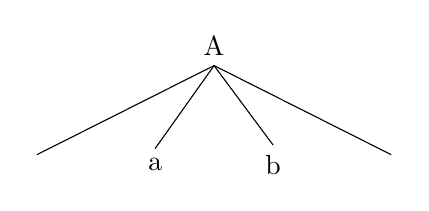
\begin{tikzpicture}
		\node {A}
		child { node{ }}
		child {node {a}}
		child {node {b}}
		child {node { }};
	\end{tikzpicture}
\end{minipage}\hfill
\begin{minipage}{0.48\textwidth}
\centering
	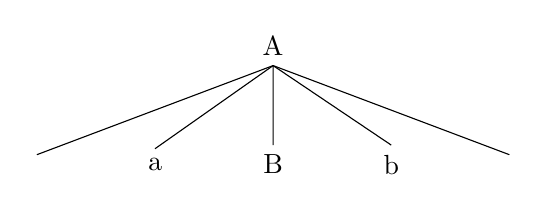
\begin{tikzpicture}
		\node {A}
		child { node{ }}
		child {node {a}}
		child {node {B}}
		child {node {b}}
		child {node { }};
   \end{tikzpicture}
\end{minipage}\hfill
\end{figure}
\end{frame}



\begin{frame}{Definirea relaţiilor de precedență operator}

\textbf{$a <_{o} b$ $\Leftrightarrow$ $\exists \ A \rightarrow \alpha a B\beta \in P$ și $B \Rightarrow^{+} b \gamma$ sau B $\Rightarrow^+ C b\gamma$}
\newline

unde $a,b \in \Sigma$, $A,B,C \in V_N$ și $\alpha, \beta \in V^*$

și se scrie $a <_{o}$ $FIRST\sim^+$(B)
\newline

($FIRST\sim^+$ = terminalul care apare pe prima poziţie sau terminalul care apare pe a doua poziţie, dacă pe prima este un neterminal)

\begin{figure}[!htb]
\begin{minipage}{0.48\textwidth}
\centering
	\begin{tikzpicture}
		\node {A}
		child { node{ }}
		child {node {a}}
		child {
				node {B}
  				child {node {b}}
  				child {node { }}
	  			}
		child {node { }};
	\end{tikzpicture}
\end{minipage}\hfill
\begin{minipage}{0.48\textwidth}
\centering
	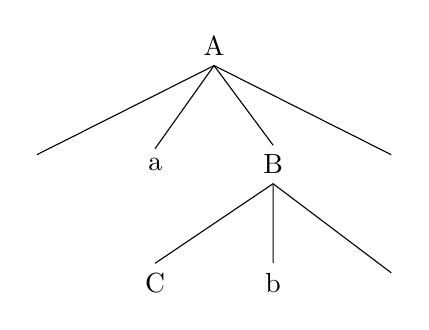
\begin{tikzpicture}
		\node {A}
		child { node{ }}
		child {node {a}}
		child {
				node {B}
				child {node {C}}
  				child {node {b}}
  				child {node { }}
	  			}
		child {node { }};
   \end{tikzpicture}
\end{minipage}\hfill
\end{figure}
\end{frame}



\begin{frame}{Definirea relaţiilor de precedență operator}
\textbf{$a >_{o} b$ $\Leftrightarrow \exists \  A \rightarrow \alpha B b\beta \in P$ și $B \Rightarrow^{+} \gamma a$ sau $B \Rightarrow^{+} \gamma a C$}
\newline

unde $a,b \in \Sigma$, $A,B,C \in V_N$ și $\alpha, \beta \in V^*$

și se scrie $LAST\sim^+$ (B)$ >_{o}$ b
\newline

($LAST\sim^+$  =  terminalul care apare pe ultima poziţie sau terminalul care apare pe penultima poziţie, dacă pe ultima este un neterminal)

\begin{figure}[!htb]
\begin{minipage}{0.48\textwidth}
\centering
  	\begin{tikzpicture}
		\node {A}
		child { node{ }}
		child {
				node {B}
  				child {node { }}
  				child {node {a}}
	  			}
	    child { node{b}}
		child {node { }};
	   \end{tikzpicture}
\end{minipage}\hfill
\begin{minipage}{0.48\textwidth}
\centering
  	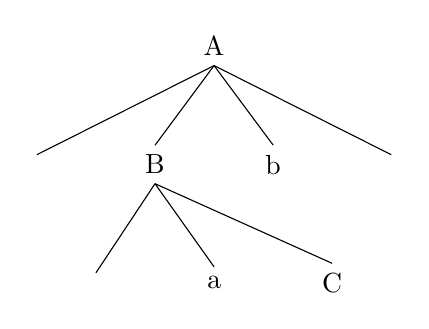
\begin{tikzpicture}
		\node {A}
		child { node{ }}
		child {
				node {B}
				child [missing]{}
				child {node { }}
  				child {node {a}}
  				child {node {C}}
	  			}
	    child {node {b}}
		child {node { }};
  	\end{tikzpicture}
\end{minipage}\hfill
\end{figure}
\end{frame}



\begin{frame}{Definirea relaţiilor de precedență operator}
$ \$ <_o a \Leftrightarrow S \Rightarrow^*  a \alpha$ sau $S \Rightarrow^* A a \alpha$
\newline


\$ este mai mic decât orice terminal care apare pe prima poziţie sau pe a doua, dacă pe prima este un neterminal, în formele propoziționale
\newline

$ a >_o \$ \Leftrightarrow S \Rightarrow^*  \alpha a$ sau $ S \Rightarrow^* \alpha a A$
\newline 

este mai mare decât \$ orice terminal care apare pe ultima poziţie sau pe penultima, dacă pe ultima este un neterminal, în formele propoziționale
\end{frame}



\begin{frame}{Definirea relaţiilor de precedență operator}
\begin{itemize}
\item
la fel ca şi la calculul mulțimilor $FIRST^+$ şi $FALLOW^+$ de la analiza LL(1), şi în cazul mulţimilor $FIRST\sim^+$ şi $LAST\sim~^+$ de la precedenţa operator se merge (în adâncime) până la nivelul maxim posibil
\item
e.g. dacă, în cazul relaţiei de precedenţă operator mai mic, se află un neterminal pe prima poziţie, atunci se ia terminalul de după, dar se și continuă aplicând pe $FIRST\sim^+$ și pentru acel neterminal
\item
analog şi în cazul relaţiei de precedenţă operator mai mare
\end{itemize}
\end{frame}



\begin{frame}{Analiza sintactică bazată pe precedenţa operator}

Etapele analizei sintactice bazate pe precedența operator:

\begin{itemize}
\item
Construirea analizorului sintactic bazat pe precedența operator:

\begin{itemize}
\item
Modificarea gramaticii astfel încât să respecte condițiile cerute pentru gramaticile operator
\item
Calcularea relațiile de precedență operator (pe baza mulțimilor $FIRST\sim^+$ sau $LAST\sim^+$) 
\item
Construirea matricei de precedență operator
\item
Implementarea analizorului bazat pe relațiile de precedență operator
\end{itemize}

\item
Analiza propriu-zisă a unei propoziții
\end{itemize}

\end{frame}



\begin{frame}{Matricea de precedență operator}
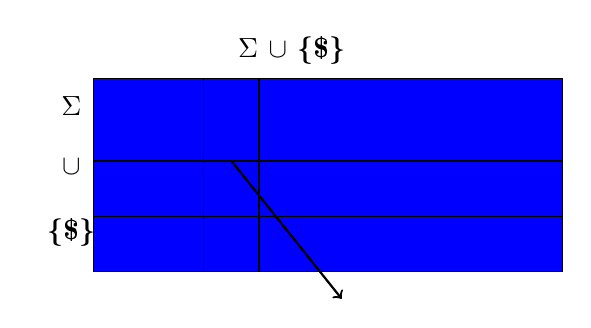
\begin{tikzpicture}[x=0.7cm, y=0.7cm]
\node at (-1,6) {\textbf{ $\Sigma$ $\cup$ \{\textdollar\}}};
\draw[black,fill=blue] (-4.5,5.5) rectangle (-2.5,4);
\draw[black,fill=blue] (-2.5,5.5) rectangle (-1.5,4);
\draw[black,fill=blue] (-1.5,5.5) rectangle (4,4);
\draw[black,fill=blue] (-4.5,3) rectangle (-2.5,4);
\draw[black,fill=blue] (-2.5,3) rectangle (-1.5,4);
\draw[black,fill=blue] (-1.5,3) rectangle (4,4);
\draw[black,fill=blue] (-4.5,2) rectangle (-2.5,4);
\draw[black,fill=blue] (-2.5,2) rectangle (-1.5,4);
\draw[black,fill=blue] (-1.5,2) rectangle (4,4);
\node at (-5,5) {\textbf{ $\Sigma$ }};
\node at (-5,3.9) {\textbf{ $\cup$ }};
\node at (-5,2.7) {\textbf{ \{\textdollar\} }};
\draw[black,fill=blue] (-4.5,2) rectangle (-2.5,3);
\draw[black,fill=blue] (-2.5,2) rectangle (-1.5,3);
\draw[black,fill=blue] (-1.5,2) rectangle (4,3);
\draw [thick, ->] (-2,4) -- (0,1.5) {};
\end{tikzpicture}

\begin{itemize}
\item
relația de precedență operator existentă între terminalul de pe linia i și terminalul de pe coloana j
\item
în celula corespunzătoare perechii ($\$, \$$) relația este "accept" - propoziția este acceptată
\item
în toate celulele care rămân necompletate relația este "error" - propoziția nu este acceptată
\end{itemize}
\end{frame}



\begin{frame}{Algoritmul de analiză pe baza matricei de precedență operator}
\begin{tabbing}
ISI $\leftarrow$ 0 \\

repetă \= \\

\> dacă ST(IST) = \$ și SI(ISI) = \$ atunci propoziția este acceptată \\

\> altfel \= \+ \\

\> a $\leftarrow$ ST(IST) \\

\> b $\leftarrow$ SI(ISI) \\

\> dacă \= $a <_o b$ sau $a =_o b$ atunci \+ \\

\> shift b în stivă \\

\> ISI $\leftarrow$ ISI + 1 \- \\

\> altfel dacă $a >_o b$ atunci  \\

\> repetă \= \+ \\

\> scoate un terminal din stivă până când \\

\> ST(IST) $<_o$ decât ultimul terminal scos din stivă \\

altfel eroare \\
\end{tabbing}
\end{frame}



\begin{frame}{Exemplu}
Fie gramatica G=$\langle \Sigma, V_N, E, P \rangle$, unde:

\begin{itemize}
\item
$\sum$=\{+,*,(,),a\}
\item
$V_N$=\{E,T,F,S,D\}
\item
E
\item
$P$=\{

\hspace{1cm} $E \rightarrow E+T$
\\
\hspace{1cm} $E \rightarrow T$
\\
\hspace{1cm} $T \rightarrow T*F$
\\
\hspace{1cm} $T \rightarrow F$
\\
\hspace{1cm} $F \rightarrow S E D$
\\
\hspace{1cm} $F \rightarrow a$
\\
\hspace{1cm} $S \rightarrow ($
\\
\hspace{1cm} $D \rightarrow )$
\\
\}
\end{itemize}

Să se analizeze sintactic propoziția $\$(a+(a+a)*a)\$$, folosind modelul automatului finit cu stivă.
\end{frame}



\begin{frame}{Exemplu}
Gramatica dată nu este o gramatică operator deoarece:
\begin{itemize}
\item
are terminale inutile ($E \rightarrow T$, $T \rightarrow F$)
\item
în partea dreaptă a unor reguli de producție există neterminale unul lângă celălalt ($F \rightarrow S E D$)
\item
prin urmare, pentru a construi un analizor sintactic ascendent bazat pe relațiile de precedență operator, \textbf{gramatica trebuie transformată într-o gramatică operator}
\end{itemize}
\end{frame}



\begin{frame}{Exemplu}
Gramatica modificată este G=$\langle \Sigma, V_N, F, P \rangle$, unde:

\begin{itemize}
\item
$\sum$=\{+,*,(,),a\}
\item
$V_N$=\{F\}
\item
F
\item
$P$=\{

\hspace{1cm} 1. F $\rightarrow$ F+F

\hspace{1cm} 2. F $\rightarrow$ F*F				

\hspace{1cm} 3. F $\rightarrow$ (F)				

\hspace{1cm} 4. F $\rightarrow$ a

\}
\end{itemize}

\end{frame}



\begin{frame}{Exemplu}
Se calculează relațiile de precedență operator:
\newline

(1) $+ <_o FIRST\sim^+(F)$

(1) $LAST\sim^+(F) >_o +$
\newline

(2) $* <_o FIRST\sim^+(F)$

(2) $LAST\sim^+(F) >_o *$
\newline

(3) $( =_o )$

(3) $( <_o FIRST\sim^+(F)$

(3) $LAST\sim^+(F) >_o )$
\newline

$\$ <_o FIRST\sim^+(F)$

$LAST\sim^+(F) >_o \$$
\end{frame}



\begin{frame}{Exemplu}
Calculând mulțimile $FIRST\sim^+$ și $LAST\sim^+$ se obține:
\newline

$LAST\sim^+(F) = \{ +, *, ), a \}$

$FIRST\sim^+(F) = \{ +, *, (, a \}$
\end{frame}



\begin{frame}{Exemplu}
Atunci, relațiile de precedență operator ar fi:
\newline

(1) $+ <_o FIRST\sim^+(F)$ \hspace{1cm} și $FIRST\sim^+(F) = \{ +, *, (, a \}$
\newline

(1) $LAST\sim^+(F) >_o +$ \hspace{1cm} și $LAST\sim^+(F) = \{ +, *, ), a \}$
\newline

$\blacktriangleright + <_o + \qquad + >_o +$\\
$\blacktriangleright + <_o * \qquad * >_o +$\\
$\blacktriangleright + <_o ( \qquad ) >_o +$\\
$\blacktriangleright + <_o a \qquad a >_o +$

\end{frame}



\begin{frame}{Exemplu}
(2) $* <_o FIRST\sim^+(F)$ \hspace{1cm} și $FIRST\sim^+(F) = \{ +, *, (, a \}$
\newline

(2) $LAST\sim^+(F) >_o *$ \hspace{1cm} și $LAST\sim^+(F) = \{ +, *, ), a \}$
\newline

$\blacktriangleright * <_o + \qquad + >_o *$\\
$\blacktriangleright * <_o * \qquad * >_o *$\\
$\blacktriangleright * <_o ( \qquad ) >_o *$\\
$\blacktriangleright * <_o a \qquad a >_o *$

\end{frame}



\begin{frame}{Exemplu}
$\blacktriangleright ( =_o )$
\newline

(3) $( <_o FIRST\sim^+(F)$ \hspace{1cm} și $FIRST\sim^+(F) = \{ +, *, (, a \}$
\newline

(3) $LAST\sim^+(F) >_o )$ \hspace{1cm} și $LAST\sim^+(F) = \{ +, *, ), a \}$
\newline

$\blacktriangleright ( <_o + \qquad + >_o )$\\
$\blacktriangleright ( <_o * \qquad * >_o )$\\
$\blacktriangleright ( <_o ( \qquad ) >_o )$\\
$\blacktriangleright ( <_o a \qquad a >_o )$
\end{frame}



\begin{frame}{Exemplu}
$\$ <_o FIRST\sim^+(F)$ \hspace{1cm} și $FIRST\sim^+(F) = \{ +, *, (, a \}$
\newline

$LAST\sim^+(F) >_o \$$ \hspace{1cm} și $LAST\sim^+(F) = \{ +, *, ), a \}$
\newline

$\blacktriangleright \$ <_o + \qquad + >_o \$$\\
$\blacktriangleright \$ <_o * \qquad * >_o \$$\\
$\blacktriangleright \$ <_o ( \qquad ) >_o \$$\\
$\blacktriangleright \$ <_o a \qquad a >_o \$$
\end{frame}



\begin{frame}{Exemplu}
Se construiește matricea de precedență:
\newline 

\begin{figure}[h]
\centering
\begin{tabular}{ | p{0.5cm} | p{0.5cm} | p{0.5cm} | p{0.5cm} | p{0.5cm} | p{0.5cm} | p{1cm} | }
\hline
	 & +   & *   & ( & ) & a & \$   \\
	 & & & & & & \\
\hline
	+& <,> & <,> & < & > & < & >    \\
	& & & & & & \\
\hline
	*& <,> & <,> & < & > & < & >    \\
	& & & & & & \\
\hline
	(& < & < & < & = & < &   \\
	& & & & & & \\
\hline
	)& > & > &	& > & & >  \\
	& & & & & & \\
\hline
	a& > & > & & > &  	& >  \\
	& & & & & & \\
\hline
	\$& < &	< & < &	& <	& accept  \\
	& & & & & & \\
\hline
\end{tabular}
\end{figure}
\end{frame}



\begin{frame}{Ambiguitatea limbajelor}
\begin{itemize}
\item
dacă un limbaj L(G) este un \textbf{limbaj ambiguu}, atunci există propoziții ale acestui limbaj pentru care \textbf{se pot construi doi sau mai mulţi arbori sintactici distincți}
\item
dacă un limbaj L(G) este ambiguu, atunci nu este obligatoriu ca pentru toate propozițiile sale să se poată construi mai mulți arbori sintactici distincți
\item
în cazul unui limbaj ambiguu, calculul relațiilor de precedență operator în baza gramaticii care îl definește va duce la situația:
\begin{itemize}
\item
\textbf{între aceleași două terminale vor exista două relații de precedență operator diferite}
\end{itemize}
\end{itemize}
\end{frame}



\begin{frame}{Ambiguitatea limbajelor}

\begin{itemize}
\item
pentru propoziţia \textbf{"a+a+a"} se pot construi doi arbori sintactici distincți:
\end{itemize}

\begin{figure}[H]
\begin{minipage}[c][1\width]{0.3\textwidth}
\centering
\caption{$+ >_o +$ - asociativitate stânga}
      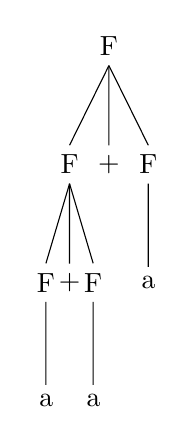
\begin{tikzpicture}
\node {F}[sibling distance=5mm]
	child{node{F}[sibling distance=3mm]
		child{node{F}
			child{node{a}}}
		child{node{+}}
		child{node{F}
			child{node{a}}}}
	child{node{+}}
	child{node{F}
		child{node{a}}}
;
      \end{tikzpicture}
\end{minipage}
\begin{minipage}[c]{0.4\textwidth} 
\centering
\caption{$+ <_o +$ - asociativitate dreapta}
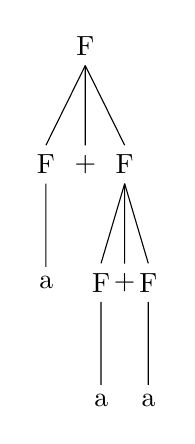
\begin{tikzpicture}
\node {F}[sibling distance=5mm]
	child{node{F}
		child{node{a}}}
	child{node{+}}
	child{node{F}[sibling distance=3mm]
		child{node{F}
			child{node{a}}}
		child{node{+}}
		child{node{F}
			child{node{a}}}}
;
\end{tikzpicture}
\end{minipage}
\end{figure}

\end{frame}



\begin{frame}{Ambiguitatea limbajelor}

\begin{itemize}
\item
la fel, pentru propoziţia \textbf{"a*a*a"} se pot construi doi arbori sintactici distincți:
\end{itemize}

\begin{figure}[H]
\begin{minipage}[c][1\width]{0.3\textwidth}
\centering
\caption{$* >_o *$ - asociativitate stânga}
      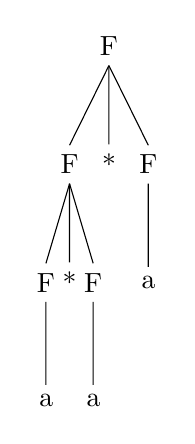
\begin{tikzpicture}
\node {F}[sibling distance=5mm]
	child{node{F}[sibling distance=3mm]
		child{node{F}
			child{node{a}}}
		child{node{*}}
		child{node{F}
			child{node{a}}}}
	child{node{*}}
	child{node{F}
		child{node{a}}}
;
      \end{tikzpicture}
\end{minipage}
\begin{minipage}[c]{0.4\textwidth} 
\centering
\caption{$* <_o *$ - asociativitate dreapta}
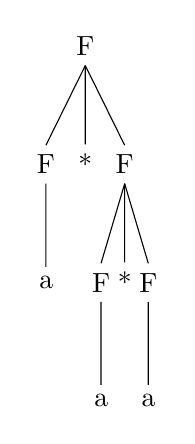
\begin{tikzpicture}
\node {F}[sibling distance=5mm]
	child{node{F}
		child{node{a}}}
	child{node{*}}
	child{node{F}[sibling distance=3mm]
		child{node{F}
			child{node{a}}}
		child{node{*}}
		child{node{F}
			child{node{a}}}}
;
\end{tikzpicture}
\end{minipage}
\end{figure}

\end{frame}



\begin{frame}{Ambiguitatea limbajelor}

\begin{itemize}
\item 
de asemenea, pentru propoziţia \textbf{"a+a*a"} se pot construi doi arbori sintactici distincți:
\end{itemize}

\begin{figure}[H]
\begin{minipage}[c][1\width]{0.3\textwidth}
\centering
\caption{$+ >_o *$ - adunarea are prioritate}
      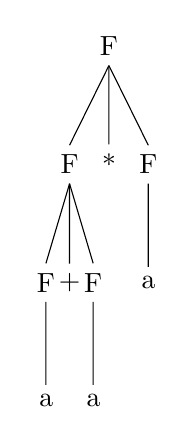
\begin{tikzpicture}
\node {F}[sibling distance=5mm]
	child{node{F}[sibling distance=3mm]
		child{node{F}
			child{node{a}}}
		child{node{+}}
		child{node{F}
			child{node{a}}}}
	child{node{*}}
	child{node{F}
		child{node{a}}}
;
      \end{tikzpicture}
\end{minipage}
\begin{minipage}[c]{0.4\textwidth} 
\centering
\caption{$+ <_o *$ - înmulțirea are prioritate}
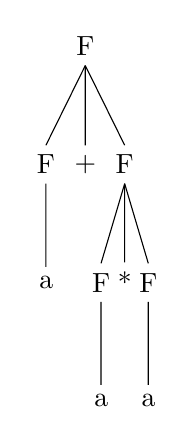
\begin{tikzpicture}
\node {F}[sibling distance=5mm]
	child{node{F}
		child{node{a}}}
	child{node{+}}
	child{node{F}[sibling distance=3mm]
		child{node{F}
			child{node{a}}}
		child{node{*}}
		child{node{F}
			child{node{a}}}}
;
\end{tikzpicture}
\end{minipage}
\end{figure}

\end{frame}



\begin{frame}{Ambiguitatea limbajelor}
\begin{itemize}
\item
în aceste cazuri, trebuie stabilită care este precedența și asociativitatea operatorilor
\item
pentru acest exemplu, se va stabili că:
\begin{itemize}
\item
\textbf{adunarea este asociativă la stânga}
\begin{itemize}
\item
se va păstra relația $+ >_o +$
\end{itemize}
\item
\textbf{înmulțirea este asociativă la stânga}
\begin{itemize}
\item
se va păstra relația $* >_o *$
\end{itemize}
\item
\textbf{înmulțirea are precedența mai mare decât adunarea}
\begin{itemize}
\item
se vor păstra relațiile $+ <_o *$ și $* >_o +$
\end{itemize}
\end{itemize}
\end{itemize}
\end{frame}



\begin{frame}{Exemplu}
Prin urmare, matricea de precedență va fi:
\newline

\begin{figure}[h]
\centering
\begin{tabular}{ | p{0.5cm} | p{0.5cm} | p{0.5cm} | p{0.5cm} | p{0.5cm} | p{0.5cm} | p{1cm} | }
\hline
	& +	& *		& (		& )		& a 	& \$  \\
	& & & & & & \\
\hline
	+& >	& <	& <	& >		& <	& >  \\
	& & & & & & \\
\hline
	*& >		& >	& <		& >		& < 	& >  \\
	& & & & & & \\
\hline
	(& <		& <		& <		& =		& < 	&   \\
	& & & & & & \\
\hline
	)& >		& >		& 		& >		&  	& >  \\
	& & & & & & \\
\hline
	a& >		& >	& 	& >		&  	& >  \\
	& & & & & & \\
\hline
	\$& <		&<	& <	& 	&  <	& accept  \\
	& & & & & & \\
\hline
\end{tabular}
\end{figure}
\end{frame}



\begin{frame}{Exemplu}

(q, \$,(a+(a+a)*a)\$,$\epsilon$)
\newline

$\vdash^{d}$ (q, \$(,a+(a+a)*a)\$,$\epsilon$) 
\newline

$\vdash^{d}$ (q, \$(a,+(a+a)*a)\$,$\epsilon$)  
\newline

$\vdash^{r}$ (q, \$(F,+(a+a)*a)\$,4)  
\newline

$\vdash^{d}$ (q, \$(F+,(a+a)*a)\$,4)  
\newline

$\vdash^{d}$ (q, \$(F+(,a+a)*a)\$,4)  
\newline

$\vdash^{d}$ (q, \$(F+(a,+a)*a)\$,4)  
\newline

$\vdash^{r}$ (q, \$(F+(F,+a)*a)\$,44)  

\end{frame}



\begin{frame}{Exemplu}

$\vdash^{d}$ (q, \$(F+(F+,a)*a)\$,44)
\newline

$\vdash^{d}$ (q, \$(F+(F+a,)*a)\$,44)
\newline

$\vdash^{r}$ (q, \$(F+(F+F,)*a)\$,444)
\newline

$\vdash^{r}$ (q, \$(F+(F,)*a)\$,4441)
\newline

$\vdash^{d}$ (q, \$(F+(F),*a)\$,4441)
\newline

$\vdash^{r}$ (q, \$(F+F,*a)\$,44413)
\newline

$\vdash^{d}$ (q, \$(F+F*,a)\$,44413)
\newline

$\vdash^{d}$ (q, \$(F+F*a,)\$,44413)
\newline

$\vdash^{r}$ (q, \$(F+F*F,)\$,444134)
\newline

\end{frame}



\begin{frame}{Exemplu}

$\vdash^{r}$ (q, \$(F+F,)\$,4441342)
\newline

$\vdash^{r}$ (q, \$(F+F,)\$,4441342)
\newline

$\vdash^{r}$ (q, \$(F,)\$,44413421)
\newline

$\vdash^{d}$ (q, \$(F),\$,44413421)
\newline

$\vdash^{r}$ (q, \$F,\$,444134213)
\newline

$\vdash^{r}$ (a, \$F,\$,444134213)


\end{frame}



\begin{frame}{Exercițiu}
Fie gramatica G=$\langle \Sigma, V_N, <instructiune>, P \rangle$, unde:

\begin{itemize}
\item
$\sum$=\{for,to,step,let,call,i,(,),,,=,*,**\}
\item
$V_N$=\{$<instructiune>$, $<atribuire>$, $<lista>$, $<expresie>$\}
\item
$<instructiune>$
\item
$P$=\{

$<instructiune> \rightarrow for <atribuire> to <expresie> [ step <expresie> ]$

$<instructiune> \rightarrow let <atribuire>$

$<instructiune> \rightarrow call \ i \ (<lista>)$

$<lista> \rightarrow i \ | \ i, <lista>$

$<atribuire> \rightarrow i = <expresie>$

$<expresie> \rightarrow i * <expresie> | i** <expresie> | i$

\}
\end{itemize}
Să se construiască un analizor sintactic ascendent bazat pe relațiile de precedență operator.
\end{frame}



\begin{frame}{Întrebări recapitulative}
\begin{itemize}
\item
Fie $AP1=(Q, \Sigma, \Gamma, f, q_0, z_0, F)$ un automat finit cu stivă care implementează analiza sintactică descendentă pentru gramatica $G=(\Sigma, V_N, S, P)$ și fie $AP2=(Q', \Sigma ', \Gamma ', f', q_0 ', z_0 ', F')$ un automat finit cu stivă care implementează analiza sintactică ascendentă pentru aceeași gramatică. Arătați care sunt diferențele dintre elementele care definesc AP1 și cele care îl definesc pe AP2 și explicați.
\newline

\item
Explicați de ce este nedeterminist algoritmul general de analiză sintactică ascendentă.
\newline

\item
Explicați rolul relației de precedență operator mai mare în analiza sintactică corespunzătoare.

\end{itemize}
\end{frame}



\begin{frame}{Întrebări recapitulative}
\begin{itemize}
\item
Enumerați și explicați diferențele dintre automatul finit cu stivă definit pentru analiza sintactică descendentă și automatul finit cu stivă definit pentru analiza sintactică ascendentă.
\newline

\item
Explicați care este diferența dintre configurația inițială a automatului finit cu stivă pentru analiza sintactică LL(1) și pentru analiza sintactică bazată pe precedența operator.
\newline

\item
Explicați cum rezolvă analiza sintactică bazată pe relațiile de precedență operator nedeterminismul algoritmului generic de analiză sintactică ascendentă.
\newline

\end{itemize}
\end{frame}



%////////////////////////////////////////////////



\begin{frame}{Alte gramatici}
G=$\langle \Sigma, V_N, <IF logic>, P \rangle$, unde:

\begin{itemize}
\item
$\sum$=\{n,IF,(,),GOTO,i,=,+,.EQ.\}
\item
$V_N$=\{$<IF logic>$, $<IF neetichetat>$, $<expresie-logica>$, $<instructiune>$, $<expresie-aritmetica>$, $<operator-logic>$\}
\item
$<IF logic>$
\item
$P$=\{

$<IF logic> \rightarrow n <IF neetichetat> | <IF neetichetat> $

$<IF neetichetat> \rightarrow IF ( <expresie-logica> ) <instructiune>$

$<instructiune> \rightarrow GOTO \ n $

$<instructiune> \rightarrow i =  n <expresie-aritmetica>$

$<expresie-logica> \rightarrow <expresie-aritmetica> <operator-logic> <expresie-aritmetica>$

$<expresie-aritmetica> \rightarrow <expresie-aritmetica> + i \  | \ i$

$<operator-logic> \rightarrow .EQ.$

\}
\end{itemize}

\end{frame}



\begin{frame}{Alte gramatici}
G=$\langle \Sigma, V_N, <instructiune>, P \rangle$, unde:

\begin{itemize}
\item
$\sum$=\{if,;,i,:=,next, sentence,+,is,<,>,,\}
\item
$V_N$=\{$<instructiune>$, $<cond>$, $<instructiune1>$, $<operand>$, $<cond>$, $<operator>$, $<oprel>$, $<zona>$\}
\item
$<instructiune>$
\item
$P$=\{

$<instructiune> \rightarrow <iif> \ | \ <imove>$

$< iif > \rightarrow if <cond> ; <instructiune1> [else < instructiune1> ]$

$< instructiune1 > \rightarrow i := <operand> | next \ sentence  $

$<cond> \rightarrow <operand> <operator> <operand>$

$<operand> \rightarrow i |  <operand> +  i$

$<operator> \rightarrow is <oprel> |  <oprel>$

$<oprel> \rightarrow < | > $

$<imove> \rightarrow move <zona> | to <zona>$

$<zona> \rightarrow i | <zona> , i$

\}
\end{itemize}

\end{frame}



\begin{frame}{Alte gramatici}
G=$\langle \Sigma, V_N, <instructiune>, P \rangle$, unde:

\begin{itemize}
\item
$\sum$=\{if,then,else,i,:=,.or.,.and.,(,),.not. \}
\item
$V_N$=\{$<instructiune>$, $<expresie>$, $<atribuire>$, $<termen>$, $<factor>$ \}
\item
$<instructiune>$
\item
$P$=\{

$<instructiune> \rightarrow if <expresie> then <atribuire> [else < atribuire> ]  $

$<atribuire> \rightarrow i := <expresie > $

$<expresie> \rightarrow <expresie> .or. <termen> | <termen> $

$<termen> \rightarrow <termen> .and. <factor> | <factor>$

$<factor> \rightarrow i | (<expresie>) | .not. <factor>$

\}
\end{itemize}

\end{frame}



\begin{frame}{Alte gramatici}
G=$\langle \Sigma, V_N, <instructiune>, P \rangle$, unde:

\begin{itemize}
\item
$\sum$=\{if,then,else,=,+,i,(,),, \}
\item
$V_N$=\{$<instructiune>$, $<expresie>$, $<atribuire>$, $<variabila>$, $<lista>$ \}
\item
$<instructiune>$
\item
$P$=\{

$<instructiune> \rightarrow if <expresie> then <atribuire> [else < atribuire > ] \ | <atribuire>$

$<atribuire> \rightarrow <variabila> = <expresie > $

$<expresie> \rightarrow <variabila> | <expresie> + <variabila> $

$<varibila> \rightarrow i \ | \ i (<lista>)$

$<lista> \rightarrow i \ | <lista> , i $

\}
\end{itemize}

\end{frame}



\begin{frame}{Alte gramatici}
G=$\langle \Sigma, V_N, <instr. DO>, P \rangle$, unde:

\begin{itemize}
\item
$\sum$=\{DO,n,i,=,, \}
\item
$V_N$=\{$<instr. DO>$, $<et>$, $<expresie>$, $<var>$ \}
\item
$<instr. DO>$
\item
$P$=\{

$<instr. DO> \rightarrow <et> DO <et><expresie>$

$<instr. DO> \rightarrow DO <et> <expresie>$

$<et> \rightarrow n$

$<expresie> \rightarrow i = <lista>$

$<lista> \rightarrow <var>,<var>,<var>$

$<var> \rightarrow i$

$<var> \rightarrow n$

\}
\end{itemize}

\end{frame}



\begin{frame}{Alte gramatici}
G=$\langle \Sigma, V_N, <decl>, P \rangle$, unde:

\begin{itemize}
\item
$\sum$=\{LET,i,=,+,-,*,/,FOR,TO,STEP, CALL,,,(,) \}
\item
$V_N$=\{$<decl>$, $<decl LET>$, $<decl FOR>$, $<decl CALL>$, $<expr>$, $<term>$, $<fact>$, $<lista>$ \}
\item
$<decl>$
\item
$P$=\{

$<decl> \rightarrow <decl LET> | <decl FOR> | <decl CALL>$

$<decl LET> \rightarrow LET \ i=<expr>$

$<expr> \rightarrow <expr>+<term> | <expr>-<term> | <term>$

$<term> \rightarrow <term>*<fact> | <term>/<fact> | <fact>$

$<fact> \rightarrow i | (<expr>)$

$<decl FOR> \rightarrow FOR \ i=<expr> TO <expr> STEP <expr>$

$<decl CALL> \rightarrow CALL \ i(<lista>)$

$<lista> \rightarrow i | <lista>, i$

\}
\end{itemize}

\end{frame}



\begin{frame}{Alte gramatici}
G=$\langle \Sigma, V_N, <instr>, P \rangle$, unde:

\begin{itemize}
\item
$\sum$=\{CALL,i,,,+,-,*,/,(,) \}
\item
$V_N$=\{$<instr>$, $<parametrii>$, $<expr>$, $<term>$, $<factor>$ \}
\item
$<instr>$
\item
$P$=\{

$<instr> \rightarrow CALL \ i (<parametrii>)$

$<parametrii> \rightarrow <expr> | <parametrii>, <expr>$

$<expr> \rightarrow <term> | <expr>+<term> | <expr>-<term>$

$<term> \rightarrow <factor> | <term>*<factor> | <term>/<factor>$ 

$<factor> \rightarrow i | (<expr>)$ 

\}
\end{itemize}

\end{frame}



\begin{frame}{Alte gramatici}
G=$\langle \Sigma, V_N, <prog>, P \rangle$, unde:

\begin{itemize}
\item
$\sum$=\{PROGRAM,VAR,BEGIN,END,id,;,:,INTEGER,,,:=,+,-,*,DIV,int,(,),READ,WRITE,FOR,DO,TO \}
\item
$V_N$=\{$<prog>$, $<prog-name>$, $<dec-list>$, $<stmt-list>$, $<dec>$, $<id-list>$, $<type>$, $<stmt>$, $<assign>$, $<read>$, $<write>$, $<for>$, $<exp>$, $<term>$, $<factor>$ \}
\item
$<prog>$
\item
$P$=\{

\end{itemize}

\end{frame}



\begin{frame}{Alte gramatici}

1. $<prog> \rightarrow PROGRAM <prog-name> VAR <dec-list> BEGIN <stmt-list> END. $

2. $<prog-name> \rightarrow id$ 

3. $<dec-list> \rightarrow <dec> | <dec-list> ; <dec> $

4. $<dec> \rightarrow <id-list> : <type> $

5. $<type> \rightarrow INTEGER $

6. $<id-list> \rightarrow id | <id-list> , id $

\end{frame}



\begin{frame}{Alte gramatici}

7. $<stmt-list> \rightarrow <stmt> | <stmt-list> ; <stmt> $

8. $<stmt> \rightarrow <assign> | <read> | <write> | <for> $

9. $<assign> \rightarrow id := <exp> $

10. $<exp> \rightarrow <term> | <exp> + <term> | <exp> - <term> $

11. $<term> \rightarrow <factor> | <term> * <factor> | <term> DIV <factor> $

12. $<factor> \rightarrow id | int | ( <exp> ) $

\end{frame}



\begin{frame}{Alte gramatici}

13. $<read> \rightarrow READ ( <id-list> ) $

14. $<write> \rightarrow WRITE ( <id-list> ) $

15. $<for> \rightarrow FOR <index-exp> DO <body> $

16. $<index-exp> \rightarrow id := <exp> TO <exp> $

17. $<body> \rightarrow <stmt> | BEGIN <stmt-list> END $

\}
\end{frame}



\begin{frame}{Bibliografie}
\begin{itemize}
\item
R.B. Yehezkael, Course Notes on Formal Languages and Compilers, Jerusalem College of Technology

\url{http://homedir.jct.ac.il/~rafi/formcomp.pdf}

\item
Paul N. Hilfinger, Course Notes, University of California, Berkeley

\url{http://inst.eecs.berkeley.edu/~cs164/sp10/notes/notes.pdf}

\item
Gavrila Ionut, Limbaje Formale și Translatoare

\url{http://facultate.regielive.ro/cursuri/calculatoare/limbaje_formale_si_translatoare-59028.html}

\item
CIS 324: Language Design and Implementation, Operator Precedence Parsing

\url{http://homepages.gold.ac.uk/nikolaev/3246-2.doc}
\end{itemize}
\end{frame}



\end{document}